\subsection{布饶尔群的应用}

在本小节中，K 是一个体，L 是 K 上的一个伽罗瓦代数，带作用 \(\lambda: G \to \operatorname{Aut}_{K}(L)\)。我们用 n 表示 L 在 K 上的次数。我们有 \(n = \operatorname{Card}(G)\)。

定理 3. —— 设 \(\mathcal{E} = (\Gamma, \iota, \pi)\) 是 G 被 L* 的一个 \(\tau\)-扩张。代数 \(\mathbf{A}[\mathcal{E}; \mathrm{L}]\) 是中心单的，且在 K 上的次数为 \(n^2\)。此外，典范同态 \(u\)（从 L 到 \(\mathbf{A}[\mathcal{E}; \mathrm{L}]\) 的）是从 L 到 \(\mathbf{A}[\mathcal{E}; \mathrm{L}]\) 的一个极大交换子代数上的同构。

引理 12. —— a) 除 \(\{0\}\) 与 L 外，不存在 L 的任何在 G 下不变的理想。

\begin{enumerate}
\def\labelenumi{\alph{enumi})}
\setcounter{enumi}{1}
\tightlist
\item
  设 g 是 G 的一个异于单位元素的元素，并设 \(\mathfrak{a}_{g}\) 是 L 的由形如 \(x - \lambda(g)x\) 的元素（其中 x 取遍 L）所生成的理想。我们有 \(\mathfrak{a}_{g} = L\)。
\end{enumerate}

设 \(\mathscr{S}\) 是 L 的极大理想所成之集；对 \(\mathscr{S}\) 的任一子集 S，令 \(\mathfrak{a}(S) = \bigcap_{\mathfrak{m} \in S} \mathfrak{m}\)。由于环 L 是交换且半单的（VIII, 第 310 页，注 6），映射 \(W \mapsto \mathfrak{a}(W)\) 是从 \(\mathscr{S}\) 的子集所成之集到 L 的理想所成之集上的一个双射（VIII, 第 142 页，命题 9）。理想 \(\mathfrak{a}(S)\) 在 G 下不变当且仅当 S 在 G 下不变。由于 G 传递地作用于 \(\mathscr{S}\)（VIII, 第 308 页，定理 2, vi)），\(\mathscr{S}\) 的在 G 下不变的子集只有 \(\varnothing\) 与 \(\mathscr{S}\)。由于 \(\mathfrak{a}(\varnothing) = L\) 且 \(\mathfrak{a}(\mathscr{S}) = \{0\}\)，我们便证明了断言 a)。

我们用反证法证明 b)；假设我们有 \(\mathfrak{a}_g\neq \mathrm{L}\)。设 \(\mathfrak{m}\) 是 L 的一个包含 \(\mathfrak{a}_g\) 的极大理想。于是对 L 中的每个 x，我们有 \(\lambda (g)x\equiv x\bmod \mathfrak{m}\)。特别地，m 在 g 下不变，且 \(\lambda(g)\) 在体 L/m 上由恒同映射诱导。由 VIII, 第 308 页定理 2 的性质 (vi)，\(G_{m}\) 的元素 g 是平凡的，这与 b) 的假设矛盾。

我们现在证明定理 3。向量空间 \(\mathbf{A}[\mathcal{E};\mathrm{L}]\) 具有有限维数 \(\operatorname{Card}(\mathrm{G})[\mathrm{L}:\mathrm{K}] = n^2\)（在 \(\mathrm{K}\) 上；由 VIII, 第 316 页以及所设等式 \(\operatorname{Card}(\mathrm{G}) = [\mathrm{L}:\mathrm{K}] = n\)）。

设 \(\mathfrak{a}\) 是代数 \(\mathbf{A}[\mathcal{E};\mathrm{L}]\) 的一个非零双边理想。我们采用 VIII, 第 316 页的记号。每个元素 \(a\)（\(\mathbf{A}[\mathcal{E};\mathrm{L}]\) 的）都可以唯一地写成 \(a = \sum_{g\in \mathrm{G}}a_g\varepsilon_g\)，其中 \(a_g\in \mathrm{L}\) 对每个 \(g\in \mathrm{G}\) 成立；我们用 \(\Phi (a)\) 表示元素 \(g\)（\(\mathrm{G}\) 的、使得 \(a_g\neq 0\) 的）所成的集合。由 VIII, 第 316 页的公式 (32)，我们有关系式

\[
\varepsilon_ {g} \varepsilon_ {g ^ {\prime}} = c _ {\sigma} (g, g ^ {\prime}) \varepsilon_ {g g ^ {\prime}}\tag{38}
\]

对所有 \(g, g' \in \mathrm{G}\) 成立，由此推出

\[
\Phi (a \varepsilon_ {g}) = \Phi (a). g\tag{39}
\]

对每个 \(g\in \mathbf{G}\) 与每个 \(a\in \mathbf{A}[\mathcal{E};\mathrm{L}]\)。

设 \(a\) 是 \(\mathfrak{a}\) 的一个非零元素，\(\Phi(a)\) 对于包含关系为极小；由公式 (39)，如有必要，把 \(a\) 换成形如 \(a\varepsilon_{g^{-1}}\) 的元素（其中 \(g\in\Phi(a)\)），我们就可以假设我们有 \(e\in\Phi(a)\)。设 \(s\) 是 \(\Phi(a)\) 的一个异于 \(e\) 的元素。由引理 12, b)，存在 L 的一个元素 \(x\)，使得 \(a_s(x-\lambda(s)\cdot x)\neq0\)。但我们有关系式

\[
x a - a x = \sum_ {g} a _ {g} (x - \lambda (g) \cdot x) \varepsilon_ {g},\tag{40}
\]

其中求和取遍 \(\Phi(a)\) 中异于 e 的元素 g。由于 \(\Phi(a)\) 的极小性，我们得到 xa - ax = 0，但这与对 x 的选取矛盾。于是我们用反证法证明了 \(\Phi(a)\) 只含 G 的单位元素 e，从而我们有 \(a \in L\)。

于是 \(L \cap a\) 是 L 的一个不化归为 \(\{0\}\) 的理想。此外，对 L 中的每个 x，我们有 \(\varepsilon_{g}x\varepsilon_{g}^{-1} = \lambda(g) \cdot x\)，故 \(L \cap a\) 在 G 下不变。由引理 12，我们因此有 \(L \cap a = L\)，即 \(L \subset a\)。由于 L 含有 \(A[E;L]\) 的单位元素，我们有 \(a = A[E;L]\)。

由于代数 \(A[E;L]\) 在 K 上具有非零的有限维数，且它仅有的双边理想是 \(\{0\}\) 与 \(A[E;L]\)，故它是单的。

我们证明与 L 交换的每个元素 \(a\)（\(\mathbf{A}[\mathcal{E};\mathrm{L}]\) 的）都属于 L。我们把 \(a\) 写成 \(\sum_{g\in \mathrm{G}}a_g\varepsilon_g\)，其系数 \(a_{g}\) 在 L 中。对 L 中的每个 \(x\)，我们有 \(xa - ax = 0\)，而关系式 (40) 表明我们有

\[
a _ {g} (x - \lambda (g) \cdot x) = 0\tag{41}
\]

对每个 \(g \in \mathrm{G}\) 与 \(x \in \mathrm{L}\)。由引理 12，我们因此有 \(a_g = 0\)（对 \(g \neq e\)）；从而 \(a \in \mathrm{L}\)。

最后，我们来确定 \(\mathbf{A}[\mathcal{E};\mathrm{L}]\) 的中心。若 \(z\) 属于中心，则它与 \(\mathrm{L}\) 交换，从而属于 \(\mathrm{L}\)。但这时我们有

\[
0 = \varepsilon_ {g} z - z \varepsilon_ {g} = (\lambda (g) \cdot z - z) \varepsilon_ {g}
\]

对 G 的每个 g 成立。于是 z 在 L 的自同构群 \(\lambda(\mathrm{G})\) 下不变。因此按假设我们有 \(z \in K\)。

定理 4. —— 设 A 是 K 上的一个有限次数中心单代数，并设 L 是 A 的一个极大交换子代数。则存在一个 \(\tau\)-扩张 \(\mathcal{E}\)（G 被 \(\mathrm{L}^*\) 的），使得 A 同构于 \(\mathbf{A}[\mathcal{E};\mathrm{L}]\)。

不失一般性，我们可以假设 L 是 A 的一个极大交换子代数。设 \(\Gamma\) 是由 A 中满足如下条件的可逆元素 \(\gamma\) 组成的乘法群：存在 G 中的 g 使得

\[
\gamma x \gamma^ {- 1} = \lambda (g). x\tag{42}
\]

对 L 的每个元素 x 成立。若给定了 \(\gamma \in \Gamma\)，则满足这一关系的元素 g 是唯一的；我们把它记作 \(\pi(\gamma)\)。直接看出，\(\pi\) 是从 \(\Gamma\) 到 G 的一个同态，且其核等于 \(L^{*}\)。\(\pi\) 的满射性由斯科伦--诺特定理（VIII, 第 263 页，推论）得出。

如果把从 \(L^{*}\) 到 \(\Gamma\) 中的典范单射记作 \(\iota\)，那么由诸构造推出，\(\mathcal{E} = (\Gamma, \iota, \pi)\) 是一个 \(\tau\)-扩张（G 被 \(L^{*}\) 的）。设

\[
u: \mathrm{L} \to \mathbf {A} [ \mathcal {E}; \mathrm{L} ] \quad \text { and } \quad v: \Gamma \to \mathbf {A} [ \mathcal {E}; \mathrm{L} ]
\]

为诸典范同态。由 \(\mathbf{A}[\mathcal{E};\mathrm{L}]\) 的普遍性质（VIII, 第 315 页，命题 12），存在唯一的代数同态 \(f:\mathbf{A}[\mathcal{E};\mathrm{L}]\to \mathrm{A}\)，使得 \(f\circ u(x) = x\) 与 \(f\circ v(\gamma) = \gamma\)（对 \(x\in \mathrm{L}\) 与 \(\gamma \in \Gamma\)）。由于代数 \(\mathbf{A}[\mathcal{E};\mathrm{L}]\) 是单的，同态 \(f\) 是单射的。而代数 \(\mathbf{A}[\mathcal{E};\mathrm{L}]\) 的次数为 \(n^2\)（在 \(\mathbf{K}\) 上），\(\mathrm{A}\) 亦然，因为 \(\mathrm{L}\) 是 \(\mathrm{A}\) 的一个极大交换半单子代数，且我们有 \(n = [\mathrm{L}:\mathrm{K}]\)（VIII, 第 262 页，命题 3, (ii)）。于是 \(f\) 是双射。

定义 2. —— 设 \(\mathscr{S}\) 是 L 的极大理想所成之集。我们定义

\[
\operatorname{Br} (\mathrm{L} / \mathrm{K}) = \bigcap_ {\mathfrak {m} \in \mathscr {S}} \operatorname{Ker} (r _ {(\mathrm{L} / \mathfrak {m}) / \mathrm{K}}),
\]

其中 \(r_{(L/\mathfrak{m})/K} : \mathrm{Br}(K) \to \mathrm{Br}(L/\mathfrak{m})\) 是标量扩张同态（VIII, 第 281 页）。

定理 5. —— 存在一个群同构

\[
\Psi : \mathrm{Ex} _ {\tau} (\mathrm{G}, \mathrm{L} ^ {*}) \longrightarrow \mathrm{Br} (\mathrm{L} / \mathrm{K})
\]

它把一个 \(\tau\)-扩张 \(\mathcal{E}\)（G 被 \(\mathrm{L}^*\) 的）的类映为 \(\mathrm{Br}(\mathrm{L} / \mathrm{K})\) 中代数 \(\mathbf{A}[\mathcal{E};\mathrm{L}]\) 的类。

为了定义 \(\Psi\) 并验证它是双射，我们必须确立以下几点：

\begin{enumerate}
\def\labelenumi{\alph{enumi})}
\item
  若 \(\mathcal{E}\) 与 \(\mathcal{E}'\) 是两个同构的 \(\tau\)-扩张（\(G\) 被 \(L^*\) 的），则代数 \(\mathbf{A}[\mathcal{E}; L]\) 与 \(\mathbf{A}[\mathcal{E}'; L]\) 同构。
\item
  反之，若代数 \(\mathbf{A}[\mathcal{E};\mathrm{L}]\) 与 \(\mathbf{A}[\mathcal{E}';\mathrm{L}]\) 同构，则 \(\tau\)-扩张 \(\mathcal{E}\) 与 \(\mathcal{E}'\)（\(\mathrm{G}\) 被 \(\mathrm{L}^*\) 的）同构。
\item
  在 \(\mathrm{Br(L / K)}\) 的每个类中，都有一个代数 \(E\)，它包含 \(L\) 作为极大交换子代数。
\item
  若 \(\mathrm{E}\) 是 \(\mathrm{K}\) 上的一个有限次数中心单代数，它包含 \(\mathrm{L}\) 作为极大交换子代数，则存在一个 \(\tau\)-扩张 \(\mathcal{E}\)（\(\mathrm{G}\) 被 \(\mathrm{L}^*\) 的），使得 \(\mathrm{E}\) 同构于 \(\mathbf{A}[\mathcal{E};\mathrm{L}]\)。
\end{enumerate}

断言 a) 由交叉乘积的构造得出；b) 由 VIII, 第 263 页的推论得出。断言 c) 由 VIII, 第 281 页的命题 5 得出，而 d) 就是上面的定理 4。

剩下要验证 \(\Psi\) 是一个群同态；为此，只需证明：若 \(\mathcal{E}_1 = (\Gamma_1,\iota_1,\pi_1)\) 与 \(\mathcal{E}_2 = (\Gamma_2,\iota_2,\pi_2)\) 是两个 \(\tau\)-扩张，则代数 \(\mathbf{A}[\mathcal{E}_1\mathcal{E}_2;\mathrm{L}]\) 等价于代数 \(\mathbf{A}[\mathcal{E}_1;\mathrm{L}]\otimes \mathbf{A}[\mathcal{E}_2;\mathrm{L}]\)。我们把积扩张 \(\mathcal{E}_1\mathcal{E}_2\) 记作 \(\mathcal{E} = (\Gamma ,\iota ,\pi)\)。群 \(\Gamma\) 同构于同态 \(\rho\)（从 \(\mathrm{L}^*\) 到纤维积 \(\Gamma_1\times_{\mathrm{G}}\Gamma_2\)，把 \(\mu\) 映为 \((\iota_1(\mu),\iota_2(\mu)^{-1})\)）的余核。对 \(i\in \{1,2\}\)，记 \(\mathrm{A}_i = \mathbf{A}[\mathcal{E}_i;\mathrm{L}]\)。设 \(u_{i}:\mathrm{L}\to \mathrm{A}_{i}\) 与 \(v_{i}:\Gamma_{i}\rightarrow \mathrm{A}_{i}^{*}\) 为诸典范同态。我们通过诸同态 \(u_{i}\) 把 L 与它的像等同起来，这些同态使 L 成为诸 \(\mathrm{A}_i\) 的极大交换子代数。我们用 \(\mathrm{V}_i\) 表示由 \(\mathrm{A}_i\) 中的左乘定义的 L-向量空间。环 \(\mathrm{L}\otimes_{\mathrm{K}}\mathrm{A}_i^{\circ}\) 作用于 \(\mathrm{V}_i\)。由于它是单的并且在 L 上的维数为 \(n^2\)，我们得到一个从 \(\mathrm{L}\otimes_{\mathrm{K}}\mathrm{A}_i^{\circ}\) 到 \(\operatorname {End}_{\mathrm{L}}(\mathrm{V}_{i})\) 上的同构。于是环 \(\mathrm{L}\otimes_{\mathrm{K}}\mathrm{A}_1^{\circ}\otimes_{\mathrm{K}}\mathrm{A}_2^{\circ}\)（我们可以把它与 \((\mathrm{L}\otimes_{\mathrm{K}}\mathrm{A}_1^{\circ})\otimes_{\mathrm{L}}(\mathrm{L}\otimes_{\mathrm{K}}\mathrm{A}_2^{\circ})\) 等同）同构于 \(\operatorname {End}_{\mathrm{L}}(\mathrm{V}_{1}\otimes_{\mathrm{L}}\mathrm{V}_{2})\)。令 \(\mathrm{C} = \operatorname {End}_{\mathrm{A}_1^{\circ}\otimes_{\mathrm{K}}\mathrm{A}_2^{\circ}}(\mathrm{V}_1\otimes_\mathrm{L}\mathrm{V}_2)\)。由 VIII, 第 282 页的引理 3，环 C 相似于 \(\mathrm{A}_1\otimes_{\mathrm{K}}\mathrm{A}_2\)，且 \(\mathrm{L}\otimes 1\otimes 1\) 是 C 的一个极大交换子代数。对每一对 \((\gamma_{1},\gamma_{2})\in \Gamma_{1}\times \Gamma_{2}\)（满足 \(\pi_1(\gamma_1) = \pi_2(\gamma_2)\)），我们用 \(w(\gamma_1,\gamma_2)\) 表示

唯一的 \(\lambda (\pi_1(\gamma_1))\)-半线性的（II, §1, No.~13, 第 223 页）自同态，使得

\[
w (\gamma_ {1}, \gamma_ {2}) (x _ {1} \otimes x _ {2}) = v _ {1} (\gamma_ {1}) x _ {1} \otimes v _ {2} (\gamma_ {2}) x _ {2}
\]

对 \(x_{1} \in V_{1}\) 与 \(x_{2} \in V_{2}\)。我们有 \(w(\gamma_{1}, \gamma_{2}) \in \mathrm{C}^{*}\)，且 w 是从纤维积 \(\Gamma_{1} \times_{G} \Gamma_{2}\) 到 \(C^{*}\) 的一个群同态。这个同态在 \(\rho\) 的像上是平凡的，并诱导一个从 \(\Gamma\) 到 \(C^{*}\) 的同态 v。用 \(u : L \to C\) 表示由 \(u : \ell \mapsto \ell \otimes 1 \otimes 1\) 给出的态射。我们可以验证关系式

\[
u (\alpha) = v (\iota (\alpha)) \quad \text { and } \quad u (^ {\gamma} \beta) = v (\gamma) u (\beta) v (\gamma) ^ {- 1}
\]

对 \(\alpha \in \mathrm{L}^*\)、\(\beta \in \mathrm{L}\) 与 \(\gamma \in \Gamma\)。VIII, 第 315 页的命题 12 给出一个同态 \(f\)（从代数 \(\mathbf{A}[\mathcal{E};\mathrm{L}]\) 到 \(\mathrm{C}\) 的）。由于代数 \(\mathbf{A}[\mathcal{E};\mathrm{L}]\) 是单的，同态 \(f\) 是单射的。代数 \(\mathrm{C}\) 与 \(\mathbf{A}[\mathcal{E};\mathrm{L}]\) 在 \(\mathrm{K}\) 上有相同的维数，故 \(f\) 是同构。

注. —— 1) 若 L 是 K 上的一个平展代数且 G 是 L 的自同构群，则代数 \(A[E;L]\) 并不总是中心单的（例如，可取 \(L = K^{n}\) 与 \(G = S_{n}\)）。

\begin{enumerate}
\def\labelenumi{\arabic{enumi})}
\setcounter{enumi}{1}
\tightlist
\item
  我们可以如下计算一个 2-闭上链 c，它与一个被带群 G 的有限伽罗瓦扩张 L 分裂的代数 A 相伴。首先，存在一个 K-同态 \(\varphi: A \to \mathbf{M}_{m}(L)\)，其中 \([A:K] = m^{2}\)。对 \(g \in G\)，用 \(\varphi^{g}\) 表示从 A 到 \(\mathbf{M}_{m}(L)\) 的由 \(a \mapsto \varphi(g^{-1}ag)\) 给出的同态。由斯科伦--诺特定理（VIII, 第 256 页，定理 3），对每个 \(g \in G\)，存在元素 \(u_{g}\)（\(\mathbf{GL}_{m}(L)\) 的），使得
\end{enumerate}

\[
\varphi^ {g} (a) = u _ {g} \varphi (a) u _ {g} ^ {- 1}
\]

对 \(a\in \mathrm{A}\)。然后我们令

\[
c (g, g ^ {\prime}) = u _ {g} u _ {g ^ {\prime}} u _ {g g ^ {\prime}} ^ {- 1}.
\]

我们也可以定义 G 被 \(L^{*}\) 的一个扩张，其作法是使用 \(\varphi\)：我们考虑群 \(\Gamma \subset \mathbf{GL}_{m}(L)\)，它由满足如下条件的 \(\gamma\) 组成：存在 \(g \in G\) 使得

\[
\varphi^ {g} (a) = \gamma \varphi (a) \gamma^ {- 1}
\]

对每个 \(a \in \mathrm{A}\)。这个扩张的类是在 \(\Psi\) 之下 \(\mathrm{A}\) 的类（在 \(\mathrm{Br}(\mathrm{L} / \mathrm{K})\) 中的）的逆像。

推论. —— 映射 \(\Phi_{L/K} = \Theta \circ \Psi^{-1}\) 定义了一个从 \(\mathrm{Br}(\mathrm{L}/\mathrm{K})\) 到 \(\mathrm{H}^{2}(\mathrm{G}, \mathrm{L}^{*})\) 的群同构。

设 \(K'\) 是 K 的一个扩张，并设 \(\varphi: K' \to L\) 是一个 K-代数态射。由 G 中满足 \(\lambda(h) \circ \varphi = \varphi\) 的元素 h 组成的集 H 是 G 的一个子群，而 \(K'\)-代数 L（赋予 \(\lambda\) 到 H 的限制）是 \(K'\) 上的一个伽罗瓦代数。

命题 14. —— 下面的图交换：

\[
\begin{array}{c} \operatorname{Br} (\mathrm{L} / \mathrm{K}) \xrightarrow {\Phi_ {\mathrm{L} / \mathrm{K}}} \operatorname{H} ^ {2} (\operatorname{G}, \operatorname{L} ^ {*}) \\ \Biggl \downarrow^ {r _ {\mathrm{K} ^ {\prime} / \mathrm{K}}} \qquad \qquad \qquad \qquad \Biggl \downarrow^ {\operatorname{Res} _ {\mathrm{H}} ^ {\mathrm{G}}} \\ \operatorname{Br} (\mathrm{L} / \mathrm{K} ^ {\prime}) \xrightarrow {\Phi_ {\mathrm{L} / \mathrm{K} ^ {\prime}}} \operatorname{H} ^ {2} (\operatorname{H}, \operatorname{L} ^ {*})  . \end{array}
\]

这由 VIII, 第 299 页的命题 7 与 VIII, 第 317 页的命题 13 得出。

\subsection{指数与阶}

定理 6. —— 设 K 是一个交换域，并设 A 是 K 上的一个有限次数中心单代数。设 L 是 K 的一个有限次数可分扩张，它是代数 A 的一个分裂域。则 \([L:K][A]\) 在 \(\mathrm{Br}(K)\) 中为零。

存在 L 的一个扩张 M，它是 K 的一个有限次数伽罗瓦扩张（V, §10, No.~1, 第 57 页，命题 2）。A 的类 {[}A{]}（在 K 的布饶尔群中的）属于子群 Br(M/K)。设 G 是 M 在 K 上的伽罗瓦群，并设 \(\alpha\) 是 {[}A{]} 在 \(H^{2}(G,M^{*})\) 中的像（VIII, 第 321 页，推论）。设 H 是 M 在 L 上的伽罗瓦群。则 H 是 G 中指标为 {[}L:K{]} 的子群（V, §10, No.~7, 第 68 页，推论 5）。由于 \(\operatorname{Res}_{\mathrm{H}}^{\mathrm{G}}(\alpha)=\Phi_{\mathrm{M/L}}(\mathrm{A}_{(\mathrm{L})})\)（命题 14），我们有 \(\operatorname{Res}_{\mathrm{H}}^{\mathrm{G}}(\alpha)=0\)。由 VIII, 第 303 页的命题 8 推出 {[}L:K{]} \(\alpha=0\)，从而 {[}L:K{]}{[}A{]}=0。

设 K 是一个交换域，并设 A 是 K 上的一个有限次数中心单代数。则 A 同构于形如 \(\mathbf{M}_{n}(\mathrm{D})\) 的代数，其中 D 是一个中心为 K 的体，且 \([A]=[D]\)（在 \(\mathrm{Br}(K)\) 中）。D 的约化次数只依赖于 A。我们把这个约化次数称为 A 的指数。A 的指数整除 A 的约化次数。A 的阶是 A 的类在 K 的布饶尔群中的阶。

推论 1. —— 交换域上的有限次数中心单代数的阶整除其指数。

只需对一个体 D（在其中心 K 上的次数为有限的）证明这一点。设 L 是 D 的一个极大交换子域，它是 K 的一个可分扩张；我们有 \([D:K]=[L:K]^{2}\)（VIII, 第 265 页，推论 2, b) 与 c)）。于是 K 的扩张 L 是代数 D 的一个分裂域（VIII, 第 281 页，命题 5），且 \([L:K]\) 与 D 的约化次数一致。然后我们应用定理 6。

推论 2. —— 设 K 是一个交换域，并设 A 是 K 上的一个有限次数中心单代数。设 p 是一个素数。若 p 整除 A 的指数，则 p 整除 A 的阶。

我们假设素数 \(p\) 不整除 A 的阶，并证明它不整除 A 的指数。只需在 A 是一个体的情况下证明这一结果。设 L 是 K 的一个分裂 A 的有限次数伽罗瓦扩张。设 G 是 L 在 K 上的伽罗瓦群，并设 H 是 G 的一个西罗 \(p\)-子群（I, §6, No.~6, 第 78 页）。我们用 \(\mathrm{L}' = \mathrm{L}^{\mathrm{H}}\) 表示 L 中 H 的不变量所成的子域。\(\mathrm{A}_{(\mathrm{L}')}\) 的阶整除 A 的阶，从而与 \(p\) 互素。由定理 6，我们有 \([\mathrm{L}:\mathrm{L}'][\mathrm{A}_{(\mathrm{L}')}] = 0\)（在 \(\mathrm{L}'\) 的布饶尔群中）。由此推出 \([\mathrm{A}_{(\mathrm{L}')}] = 0\)，且体 \(\mathrm{L}'\) 分裂 A。然后我们应用 VIII, 第 283 页的推论 2；由此推出 A 的指数整除 \([\mathrm{L}':\mathrm{K}]\)，从而不被 \(p\) 整除。

推论 3. —— 设 p 是一个素数，并设 K 是一个特征为 p 的完全域。设 A 是 K 上的一个有限次数中心单代数。则 p 不整除 A 的指数。

我们证明 K 的布饶尔群不含阶为 p 的元素。K 的每个有限次数伽罗瓦扩张 M 都是完全域（V, §7, No.~1, 第 36 页，命题 2）。于是取 p 次幂是群 \(M^{*}\) 的一个自同构。由此推出，用 p 作乘法是群 \(\mathrm{H}^{2}(\mathrm{Gal}(\mathrm{M}/\mathrm{K}),\mathrm{M}^{*})\) 的自同构，该群同构于 \(\mathrm{Br}(\mathrm{M}/\mathrm{K})\)。

因此，{[}A{]} 的阶与 \(p\) 互素，且由推论 2，其指数不被 \(p\) 整除。

注. —— 通过考虑四元数代数的张量积，可以构造以 K 为中心、阶为 2 且指数任意大的体（参看 VIII, 第 371 页，习题 7 与 8）。

*反之，若 K 是 \(p\)-进域或有限域上形式幂级数域的一个有限伽罗瓦扩张，则 K 上的有限次数中心单代数的阶等于其指数（VIII, 第 332 页，习题 17, e)）。*

\BourbakiExercises{习题}

\begin{enumerate}
\def\labelenumi{\arabic{enumi})}
\tightlist
\item
  设 G 是一个群，Z{[}G{]} 是 G 在 Z 上的代数；我们把 G 与 Z{[}G{]} 的典范基等同起来。设 M 是一个 Z{[}G{]}-模，也就是说，一个赋予 G 的作用（保持其群结构的）的交换群。对任何整数 \(n \geqslant 0\)，用 \(C^{n}(G, M)\) 表示从 \(G^{n}\) 到 M 的映射所成的群；令 \(C^{n}(G, M) = 0\)（对 n \textless{} 0）。用下面的公式定义一个同态 \(d^{n}: C^{n}(G, M) \to C^{n+1}(G, M)\)：
\end{enumerate}

\[
\begin{array}{c} (d ^ {n} c) (g _ {0}, \ldots , g _ {n}) = g _ {0}   c (g _ {1}, \ldots , g _ {n}) + \sum_ {i = 0} ^ {n - 1} (- 1) ^ {i + 1} c (g _ {0}, \ldots , g _ {i} g _ {i + 1}, \ldots , g _ {n}) \\ \qquad \qquad \qquad \qquad \qquad \qquad \qquad \qquad \qquad \qquad \qquad \qquad + (- 1) ^ {n + 1} c (g _ {0}, \ldots , g _ {n - 1})  . \end{array}
\]

对任何整数 \(n\)，令 \(Z^n(\mathrm{G},\mathrm{M}) = \operatorname{Ker} d^n\) 与 \(B^n(\mathrm{G},\mathrm{M}) = \operatorname{Im} d^n\)。

\begin{enumerate}
\def\labelenumi{\alph{enumi})}
\tightlist
\item
  证明 \(\mathrm{B}^n (\mathrm{G},\mathrm{M})\) 包含于 \(\mathbf{Z}^n (\mathbf{G},\mathbf{M})\)。
\end{enumerate}

令 \(\mathrm{H}^{n}(\mathrm{G},\mathrm{M})=\mathrm{Z}^{n}(\mathrm{G},\mathrm{M})/\mathrm{B}^{n}(\mathrm{G},\mathrm{M})\)。群 \(\mathrm{H}^{0}(\mathrm{G},\mathrm{M})\) 是 M 中被 G 的作用固定的元素所成之集。群 \(\mathrm{Z}^{1}(\mathrm{G},\mathrm{M})\) 是映射 \(f:\mathrm{G}\to\mathrm{M}\) 所成的群，其中 f 满足 \(f(gg')=f(g)+gf(g')\)，而 \(\mathrm{B}^{1}(\mathrm{G},\mathrm{M})\) 是如下映射 f 所成的子群：存在 \(m\in M\) 使得 \(f(g)=gm-m\)（参看 I, §6, 第 148 页，习题 7）。

\begin{enumerate}
\def\labelenumi{\alph{enumi})}
\setcounter{enumi}{1}
\item
  设 N 是一个 Z{[}G{]}-模，并设 \(u : M \to N\) 是一个 Z{[}G{]}-线性映射。对每个整数 n，映射 \(c \mapsto u \circ c\) 是从 \(C^{n}(G, M)\) 到 \(C^{n}(G, N)\) 的同态，它把 \(Z^{n}(G, M)\) 映入 \(Z^{n}(G, N)\)，把 \(B^{n}(G, M)\) 映入 \(B^{n}(G, N)\)，从而诱导一个从 \(H^{n}(G, M)\) 到 \(H^{n}(G, N)\) 的同态，我们把它记作 \(H^{n}(G, u)\) 或简记作 \(H^{n}(u)\)。若 \(v : N \to P\) 是 Z{[}G{]}-模的一个同态，则我们有 \(H^{n}(v \circ u) = H^{n}(v) \circ H^{n}(u)\)。
\item
  设 \(0 \to M' \xrightarrow{\iota} M \xrightarrow{\pi} M'' \to 0\) 是 Z{[}G{]}-模的一个正合列。设 n 是一个整数，并设 \(x''\) 是 \(\mathrm{H}^{n}(\mathrm{G},\mathrm{M}'')\) 的一个元素，即元素 \(c'' \in Z^{n}(\mathrm{G},\mathrm{M}'')\) 的类。设 \(c \in \mathrm{C}^{n}(\mathrm{G},\mathrm{M})\) 满足 \(\pi \circ c = c''\)。证明存在一个元素 \(c' \in \mathrm{Z}^{n+1}(\mathrm{G},\mathrm{M}')\) 使得 \(\iota \circ c' = d^{n}(c)\)，并且 \(c'\) 在 \(\mathrm{H}^{n+1}(\mathrm{G},\mathrm{M}')\) 中的类只依赖于 \(x''\)；我们把该类记作 \(\partial^{n}(x'')\)。映射 \(\partial^{n}: \mathrm{H}^{n}(\mathrm{G},\mathrm{M}'') \to \mathrm{H}^{n+1}(\mathrm{G},\mathrm{M}')\) 是一个同态（“连接同态”）。证明序列
\end{enumerate}

\[
\dots \longrightarrow \mathrm{H} ^ {n} (\mathrm{G}, \mathrm{M} ^ {\prime}) \stackrel {{\mathrm{H} ^ {n} (\iota)}} {{\longrightarrow}} \mathrm{H} ^ {n} (\mathrm{G}, \mathrm{M}) \stackrel {{\mathrm{H} ^ {n} (\pi)}} {{\longrightarrow}} \mathrm{H} ^ {n} (\mathrm{G}, \mathrm{M} ^ {\prime \prime}) \stackrel {{\partial^ {n}}} {{\longrightarrow}} \mathrm{H} ^ {n + 1} (\mathrm{G}, \mathrm{M} ^ {\prime}) \longrightarrow \dots
\]

是正合的。

\begin{enumerate}
\def\labelenumi{\arabic{enumi})}
\setcounter{enumi}{1}
\tightlist
\item
  设 \(\varphi : \mathrm{H} \to \mathrm{G}\) 是一个群同态，M 是一个 Z{[}G{]}-模，N 是一个 Z{[}H{]}-模，并设 \(u : \mathrm{M} \to \mathrm{N}\) 是交换群的一个同态。我们说 \(\varphi\) 与 \(u\) 是相容的，如果我们有 \(u(\varphi(h)x) = hu(x)\)（对每个 \(h \in \mathrm{H}\) 与每个 \(x \in \mathrm{M}\)）。
\end{enumerate}

\begin{enumerate}
\def\labelenumi{\alph{enumi})}
\item
  对 \(n \geqslant 0\)，设 \(\varphi^{n}: H^{n} \to G^{n}\) 是由 \(\varphi\) 诱导的映射；若 \(\varphi\) 与 u 相容，则同态 \(c \mapsto u \circ c \circ \varphi^{n}\)（从 \(C^{n}(G, M)\) 到 \(C^{n}(H, N)\) 的）把 \(Z^{n}(G, M)\) 映入 \(Z^{n}(H, N)\)，把 \(B^{n}(G, M)\) 映入 \(B^{n}(H, N)\)，从而诱导一个同态 \(H^{n}(\varphi, u)\)（从 \(H^{n}(G, M)\) 到 \(H^{n}(H, N)\) 的）。
\item
  设 \(\psi : \mathrm{K} \to \mathrm{H}\) 是另一个群同态，P 是一个 Z{[}K{]}-模，并设 \(v: \mathrm{N} \to \mathrm{P}\) 是交换群的一个同态。若 \(\varphi\) 与 \(u\) 相容，且 \(\psi\) 与 \(v\) 也相容，则我们有 \(\mathrm{H}^n(\varphi \circ \psi, v \circ u) = \mathrm{H}^n(\psi, v) \circ \mathrm{H}^n(\varphi, u)\)。
\item
  考虑一个交换图
\end{enumerate}

\pandocbounded{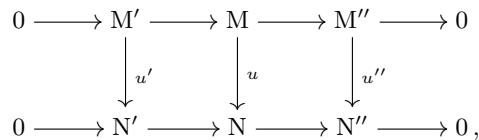
\includegraphics[keepaspectratio]{images/part002_92bb4337.jpg}}

其中第一行（相应地，第二行）是 Z{[}G{]}-模（相应地，Z{[}H{]}-模）的一个正合列，且 \(u', u, u''\) 与 \(\varphi\) 相容。证明图

\[
\begin{array}{l} \dots \longrightarrow \mathrm{H} ^ {n} (\mathrm{G}, \mathrm{M} ^ {\prime}) \longrightarrow \mathrm{H} ^ {n} (\mathrm{G}, \mathrm{M}) \longrightarrow \mathrm{H} ^ {n} (\mathrm{G}, \mathrm{M} ^ {\prime \prime}) \longrightarrow \mathrm{H} ^ {n + 1} (\mathrm{G}, \mathrm{M} ^ {\prime}) \longrightarrow \dots \\ \Biggl \downarrow_ {\mathrm{H} ^ {n} (\varphi , u ^ {\prime})} \qquad \Biggl \downarrow_ {\mathrm{H} ^ {n} (\varphi , u)} \qquad \Biggl \downarrow_ {\mathrm{H} ^ {n} (\varphi , u ^ {\prime \prime})} \qquad \Biggl \downarrow_ {\mathrm{H} ^ {n + 1} (\varphi , u)} \\ \dots \longrightarrow \mathrm{H} ^ {n} (\mathrm{H}, \mathrm{N} ^ {\prime}) \longrightarrow \mathrm{H} ^ {n} (\mathrm{H}, \mathrm{N}) \longrightarrow \mathrm{H} ^ {n} (\mathrm{H}, \mathrm{N} ^ {\prime \prime}) \longrightarrow \mathrm{H} ^ {n + 1} (\mathrm{H}, \mathrm{N} ^ {\prime}) \longrightarrow \dots \end{array}
\]

（其水平各行是习题 1, c) 中定义的长正合列）是交换的。

\begin{enumerate}
\def\labelenumi{\alph{enumi})}
\setcounter{enumi}{3}
\item
  例：若 H = G，则映射 u 与 \(Id_{G}\) 相容当且仅当它是 Z{[}G{]}-线性的，且我们有 \(\mathrm{H}^{n}(\mathrm{Id}_{\mathrm{G}}, u) = \mathrm{H}^{n}(\mathrm{G}, u)\)。若 N 等于 M（赋予一个 Z{[}G{]}-模结构，即由 \(\varphi\) 诱导的那一个），则同态 \(\varphi\) 与 \(1_{M}\) 相容；我们用 \(\operatorname{Res}^{q} : \mathrm{H}^{q}(\mathrm{G}, \mathrm{M}) \to \mathrm{H}^{q}(\mathrm{H}, \mathrm{M})\) 表示同态 \(\mathrm{H}^{q}(\varphi, 1_{\mathrm{M}})\)（“限制同态”）。
\item
  设 H 是 G 的一个正规子群，并设 \(M^{H}\) 是 M 中在 H 下不变的元素所成的子群（赋予由 G 的作用通过取商而诱导的 G/H 的作用）。典范满射 \(p: G \rightarrow G/H\) 与典范单射 \(j: M^{H} \rightarrow M\) 是相容的；我们用 \(\operatorname{Inf}^{q}: \operatorname{H}^{q}(\operatorname{G}/\operatorname{H}, \operatorname{M}^{\operatorname{H}}) \to \operatorname{H}^{q}(\operatorname{G}, \operatorname{M})\) 表示同态 \(\operatorname{H}^{q}(p, j)\)（“膨胀同态”）。证明序列
\end{enumerate}

\[
0 \to \mathrm{H} ^ {1} (\mathrm{G} / \mathrm{H}, \mathrm{M} ^ {\mathrm{H}}) \xrightarrow {\operatorname{Inf} ^ {1}} \mathrm{H} ^ {1} (\mathrm{G}, \mathrm{M}) \xrightarrow {\operatorname{Res} ^ {1}} \mathrm{H} ^ {1} (\mathrm{H}, \mathrm{M})
\]

是正合的。此外，若 \(\mathrm{H}^1 (\mathrm{H},\mathrm{M})\) 为零，则序列

\[
0 \to \mathrm{H} ^ {2} (\mathrm{G} / \mathrm{H}, \mathrm{M} ^ {\mathrm{H}}) \xrightarrow {\operatorname{Inf} ^ {2}} \mathrm{H} ^ {2} (\mathrm{G}, \mathrm{M}) \xrightarrow {\operatorname{Res} ^ {2}} \mathrm{H} ^ {2} (\mathrm{H}, \mathrm{M})
\]

是正合的。

¶ 3) 设 G 是一个群，M 是一个 Z{[}G{]}-模。让 G 作用在 C \(^{1}\) (G,M) 上，其作法是把 \((g,f)\in\mathrm{G}\times\mathrm{C}^{1}(\mathrm{G},\mathrm{M})\) 映为 G 上的函数 \(h\mapsto gf(g^{-1}h)\)。回顾（I, §6, 第 149 页，习题 8），M 上的一个 G-平均是一个 Z{[}G{]}-线性映射 \(\mu:C^{1}(\mathrm{G},\mathrm{M})\to\mathrm{M}\)，它满足 \(\mu(c_{x})=x\)，其中 \(c_{x}\) 表示取值 \(x\in\mathrm{M}\) 的常值函数。

\begin{enumerate}
\def\labelenumi{\alph{enumi})}
\item
  证明若 M 容许一个 G-平均，则 \(\mathrm{H}^{n}(\mathrm{G},\mathrm{M})\) 为零（对 \(n \geqslant 1\)）。（对 \(q \geqslant 1\)，设 \(h^{q}: \mathrm{C}^{q}(\mathrm{G},\mathrm{M}) \to \mathrm{C}^{q-1}(\mathrm{G},\mathrm{M})\) 是如下同态：对 G 中的 \(g_{1}, \ldots, g_{q-1}\) 与 \(c \in \mathrm{C}^{q}(\mathrm{G}, \mathrm{M})\)，把 \(h^{q}(c)(g_{1}, \ldots, g_{q-1})\) 定义为 \(\mu\) 作用于函数 \(g \mapsto c(g_{1}, \ldots, g_{q-1}, (g_{1} \cdots g_{q-1})^{-1}g)\) 所得的像。证明等式 \(h^{q+1} \circ d^{q} + d^{q-1} \circ h^{q} = 1_{\mathrm{C}^{q}(\mathrm{G}, \mathrm{M})}\)。
\item
  设 A 是一个交换群；用 \(\mathcal{F}(\mathrm{G},\mathrm{A})\) 表示从 G 到 A 的映射所成的群（赋予由 \({}^{g}f(h)=f(hg)\)（对 G 中的 g, h 与 \(\mathcal{F}(\mathrm{G},\mathrm{A})\) 中的 f）定义的 G 的作用）。对从 G 到 \(\mathcal{F}(\mathrm{G},\mathrm{A})\) 的任何映射 c，用 \(\mu(c)\) 表示从 G 到 A 的映射 \(g\mapsto c(g^{-1})(g)\)。证明 \(\mu\) 是 \(\mathcal{F}(\mathrm{G},\mathrm{A})\) 上的一个 G-平均；因此我们有 \(\mathrm{H}^{q}(\mathrm{G},\mathcal{F}(\mathrm{G},\mathrm{A}))=0\)（对 \(q\geqslant1\)）。
\item
  设 \(j: M \to \mathcal{F}(G, M)\) 是把 M 的元素 m 映为函数 \(g \mapsto gm\) 的映射，并设 \(M'\) 是它的余核。证明 j 是单射且是 Z{[}G{]}-线性的。由此推出同态 \(\partial^{q}: H^{q}(G, M') \to H^{q+1}(G, M)\) 是双射（对 \(q \geqslant 1\)）。
\item
  设 L 是交换域 K 的一个有限伽罗瓦扩张，并设 G 是它的伽罗瓦群。由 b) 与正规基定理（V, §10, No.~9, 第 73 页）推出，群 \(\mathrm{H}^{n}(\mathrm{G},\mathrm{L})\) 为零（对 \(n \geqslant 1\)）。
\end{enumerate}

¶ 4) 设 G 是一个群，H 是 G 的一个子群。对任何 Z{[}H{]}-模 N，用 \(\widetilde{N}\) 表示群 \(\operatorname{Hom}_{\mathbf{Z}[H]}(\mathbf{Z}[G], N)\)（赋予由 Z{[}G{]} 上的右 Z{[}G{]}-模结构诱导的一个 Z{[}G{]}-模结构）。

\begin{enumerate}
\def\labelenumi{\alph{enumi})}
\item
  证明 \(\widetilde{\mathbf{N}}\) 可与一个 \(\mathbf{Z}[\mathrm{G}]\)-子模等同起来，即 \(\mathcal{F}(\mathrm{G},\mathrm{N})\)（习题 3）中由映射 \(f\) 所组成的、满足 \(f(hg) = hf(g)\)（对每个 \(h\in \mathrm{H}\) 与每个 \(g\in \mathrm{G}\)）的那个子模。若 \(\mathrm{A}\) 是一个交换群，则 \(\mathbf{Z}[\mathrm{G}]\)-模 \(\widetilde{\mathcal{F}(\mathrm{H},\mathrm{A})}\) 典范同构于 \(\mathcal{F}(\mathrm{G},\mathrm{A})\)。
\item
  设 \(0 \rightarrow N' \stackrel{i}{\rightarrow} N \stackrel{p}{\rightarrow} N'' \rightarrow 0\) 是 Z{[}H{]}-模的一个正合列；序列
\end{enumerate}

\[
0 \longrightarrow \widetilde {\mathrm{N}} ^ {\prime} \xrightarrow {\operatorname{Hom} (1 , i)} \widetilde {\mathrm{N}} \xrightarrow {\operatorname{Hom} (1 , p)} \widetilde {\mathrm{N}} ^ {\prime \prime} \longrightarrow 0
\]

是正合的（注意 \(\mathbf{Z}[\mathrm{H}]\)-模 \(\mathbf{Z}[\mathrm{G}]\) 是自由的）。

\begin{enumerate}
\def\labelenumi{\alph{enumi})}
\setcounter{enumi}{2}
\tightlist
\item
  设 \(u_{N} : \widetilde{N} \to N\) 是映射 \(f \mapsto f(1)\)；它与典范单射 \(i : H \to G\) 相容（习题 2）。证明同态
\end{enumerate}

\[
\mathrm{H} ^ {q} (i, u _ {\mathrm{N}}): \mathrm{H} ^ {q} (\mathrm{G}, \widetilde {\mathrm{N}}) \to \mathrm{H} ^ {q} (\mathrm{H}, \mathrm{N})
\]

对每个 \(q \geqslant 0\) 是双射（先处理 q = 0 的情形，然后利用上述结果、习题 3, c) 以及习题 2, c)，对 q 作归纳法推理）。

\begin{enumerate}
\def\labelenumi{\alph{enumi})}
\setcounter{enumi}{3}
\item
  假设 H 在 G 中有有限指标 n。设 M 是一个 Z{[}G{]}-模，我们通过限制标量把它看作一个 Z{[}H{]}-模。设 \(f \in \widetilde{M}\)；元素 \(g^{-1}f(g)\) 只依赖于 g 的右陪集 Hg。令 \(\pi(f) = \sum_{Hg \in H \setminus G} g^{-1}f(g)\)。证明 \(\pi\) 是一个 Z{[}G{]}-线性同态（从 \(\widetilde{M}\) 到 M 的）。对任何整数 \(q \geqslant 0\)，用 \(\operatorname{Cor}^{q}: \mathrm{H}^{q}(\mathrm{H}, \mathrm{M}) \to \mathrm{H}^{q}(\mathrm{G}, \mathrm{M})\) 表示同态 \(\mathrm{H}^{q}(\pi) \circ \mathrm{H}^{q}(i, u_{\mathrm{M}})^{-1}\)（“余限制同态”）。
\item
  证明自同态 \(Cor^{q} \circ Res^{q}\)（\(H^{q}(G, M)\) 的）是乘以 n 的映射（先处理 q = 0 的情形，然后按 c) 的证明中的做法处理一般情形）。
\item
  假设 G 是有限的；证明对每个 Z{[}G{]}-模 M 与每个整数 \(q \geqslant 1\)，群 \(\mathrm{H}^{q}(\mathrm{G}, \mathrm{M})\) 被 G 的阶零化。
\end{enumerate}

\begin{enumerate}
\def\labelenumi{\arabic{enumi})}
\setcounter{enumi}{4}
\tightlist
\item
  设 G 是一个群，M 是一个不一定交换的群（赋予一个同态 \(\varphi: G \to \text{Aut}(M)\)）；对 \(g \in G\) 与 \(m \in M\)，令 \(^{g}m = \varphi(g)(m)\)。用 \(H^{0}(G, M)\) 表示 M 中被 G 的作用固定的元素所成的子群；它的单位元素称为 \(H^{0}(G, M)\) 的标记元素或特异元素。设 \(Z^{1}(G, M)\) 是映射 \(c: G \to M\) 所成之集，其中 c 满足 \(c(gh) = c(g)^{g}c(h)\)（对 G 中的 g, h）。对 \(c \in Z^{1}(G, M)\) 与 \(m \in M\)，映射 \(g \mapsto mc(g)(^g m)^{-1}\) 属于 \(Z^{1}(G, M)\)；这就定义了群 M 在 \(Z^{1}(G, M)\) 上的一个作用。商集记作 \(H^{1}(G, M)\)；它带有一个标记元素，即取值 1 的常值映射的类。若 M 是交换的，则集合 \(H^{1}(G, M)\) 与习题 1 中定义的那个重合。
\end{enumerate}

\begin{enumerate}
\def\labelenumi{\alph{enumi})}
\item
  设 N 是另一个赋予 G 的作用的群，并设 \(u: M \to N\) 是一个与 G 的作用相容的群同态。对 i = 0, 1，定义同态 \(\mathrm{H}^{i}(u): \mathrm{H}^{i}(\mathrm{G}, \mathrm{M}) \to \mathrm{H}^{i}(\mathrm{G}, \mathrm{N})\)，它们把 \(\mathrm{H}^{i}(\mathrm{G}, \mathrm{M})\) 的标记元素映为 \(\mathrm{H}^{i}(\mathrm{G}, \mathrm{N})\) 的标记元素。
\item
  设 \(0 \to M' \xrightarrow{\iota} M \xrightarrow{\pi} M'' \to 0\) 是带 G 中算子的群的一个正合列。设 \(x'' \in \mathrm{H}^0(\mathrm{G}, \mathrm{M}'')\)，并设 x 是 M 的一个元素，使得 \(\pi(x) = x''\)。证明存在一个元素 \(c' \in \mathrm{Z}^1(\mathrm{G}, \mathrm{M}')\)，使得 \(\iota \circ c'(g) = g^{-1}c(g)\)（对每个 \(g \in G\)），并且 \(c'\) 在 \(\mathrm{H}^1(\mathrm{G}, \mathrm{M}')\) 中的类只依赖于 \(x''\)；我们把该类记作 \(\partial(x'')\)。证明序列
\end{enumerate}

\[
0 \to \mathrm{H} ^ {0} (\mathrm{G}, \mathrm{M} ^ {\prime}) \xrightarrow {\mathrm{H} ^ {0} (\iota)} \mathrm{H} ^ {0} (\mathrm{G}, \mathrm{M}) \xrightarrow {\mathrm{H} ^ {0} (\pi)} \mathrm{H} ^ {0} (\mathrm{G}, \mathrm{M} ^ {\prime \prime}) \xrightarrow {\partial}
\]

\[
\mathrm{H} ^ {1} (\mathrm{G}, \mathrm{M} ^ {\prime}) \xrightarrow {\mathrm{H} ^ {1} (\iota)} \mathrm{H} ^ {1} (\mathrm{G}, \mathrm{M}) \xrightarrow {\mathrm{H} ^ {1} (\pi)} \mathrm{H} ^ {1} (\mathrm{G}, \mathrm{M} ^ {\prime \prime})
\]

是正合的（映射序列 \(G \xrightarrow{i} F \xrightarrow{p} E\)（其中集合 E 带有一个标记元素 e）称为在 F 处正合，如果 \(\operatorname{Im}(i) = p^{-1}(e)\)）。

\begin{enumerate}
\def\labelenumi{\alph{enumi})}
\setcounter{enumi}{2}
\item
  此外，假设 \(M'\) 包含在 M 的中心内。构造一个映射 \(\partial^{1}: H^{1}(G, M'') \to H^{2}(G, M')\)，使得单位元素在 \(\partial^{1}\) 下的逆像是 \(H^{1}(\pi)\) 的像。再定义群 \(H^{1}(G, M')\) 在集合 \(H^{1}(G, M)\) 上的一个作用，使得两个元素在这个作用下共轭当且仅当它们在 \(H^{1}(\pi)\) 下有相同的像。
\item
  设 K 是一个交换域，L 是 K 的一个有限伽罗瓦扩张（伽罗瓦群为 G），n 是一个整数。让 G 作用在群 \(\mathbf{GL}_{n}(\mathrm{L})\) 上，其作法是令 \(\sigma A = (\sigma(a_{ij}))\)（对 \(\sigma \in G\) 与 \(A = (a_{ij}) \in \mathbf{GL}_{n}(\mathrm{L})\)）。由 V, §10, No.~5, 第 64 页，命题 9 推出，集合 \(\mathrm{H}^{1}(\mathrm{G}, \mathbf{GL}_{n}(\mathrm{L}))\) 只含一个元素（“希尔伯特定理 90”）。
\end{enumerate}

¶ 6) 设 L 是交换域 K 的一个有限伽罗瓦扩张（伽罗瓦群为 G）。设 V 与 V' 是 K-向量空间，w（相应地，w'）是 V（相应地，V'）上一个 \((p,q)\) 型张量。从 \((V,w)\) 到 \((V',w')\) 的一个 L-同构是一个 L-线性同构 \(u:V_{(L)}\to V_{(L)}'\)，使得 \(u^{\otimes p}\otimes(^{t}u^{-1})^{\otimes q}\) 把 w 的像映为 \(w'\) 的像。我们用 \(\operatorname{Aut}_{\mathrm{L}}(\mathrm{V},w)\) 表示 \((\mathrm{V},w)\) 的 L-自同构所成的群，G 在其上通过 \(\sigma\varphi=(1_{\mathrm{V}}\otimes\sigma)\circ\varphi\circ(1_{\mathrm{V}}\otimes\sigma)^{-1}\) 作用。

\begin{enumerate}
\def\labelenumi{\alph{enumi})}
\item
  设 u 是从 \((\mathrm{V}, w)\) 到 \((\mathrm{V}^{\prime}, w^{\prime})\) 的一个 L-同构，\(\sigma\) 是 G 的一个元素；映射 \(\sigma u = (1_{\mathrm{V}^{\prime}} \otimes \sigma) \circ u \circ (1_{\mathrm{V}} \otimes \sigma)^{-1}\) 是从 \((\mathrm{V}, w)\) 到 \((\mathrm{V}^{\prime}, w^{\prime})\) 的一个 L-同构，从而 \(c(\sigma) = u^{-1} \circ \sigma u\) 是 \(\operatorname{Aut}_{\mathrm{L}}(\mathrm{V}, w)\) 的一个元素。证明映射 \(c : G \to \operatorname{Aut}_{\mathrm{L}}(\mathrm{V}, w)\) 属于 \(Z^{1}(\mathrm{G}, \operatorname{Aut}_{\mathrm{L}}(\mathrm{V}, w))\)，并且它的类 \(\theta(\mathrm{V}^{\prime}, w^{\prime})\)（在 \(H^{1}(\mathrm{G}, \operatorname{Aut}_{\mathrm{L}}(\mathrm{V}, w))\) 中的）不依赖于 u 的选取。
\item
  证明映射 \((\mathrm{V}^{\prime},t^{\prime})\mapsto\theta(\mathrm{V}^{\prime},t^{\prime})\) 定义了一个双射（从偶 \((\mathrm{V}^{\prime},w^{\prime})\)（L-同构于 \((\mathrm{V},w)\) 的）的 K-同构类所成之集到集合 \(\mathrm{H}^{1}(\mathrm{G},\mathrm{Aut}_{\mathrm{L}}(\mathrm{V},w))\) 的）。（设 c 是 \(\mathrm{Z}^{1}(\mathrm{G},\mathrm{Aut}_{\mathrm{L}}(\mathrm{V},w))\) 的一个元素，由习题 5, d) 推出 \(\mathrm{V}_{(\mathrm{L})}\) 的一个 L-自同构 f，使得 \(c(\sigma)=f^{-1}\circ^{\sigma}f\)。证明 w 在由 f 诱导的自同构下的像 \(w^{\prime}\) 在 K 上是有理的，并考虑偶 \((\mathrm{V},w^{\prime}).\)）
\end{enumerate}

* c) 例：集合 \(\mathrm{H}^1 (\mathrm{G},\mathbf{Sp}_{2n}(\mathrm{L}))\) 只含一个元素。若 Q 是 K 上的一个二次型，则集合 \(\mathrm{H}^1 (\mathrm{G},\mathbf{O}(\mathrm{Q}_{(\mathrm{L})}))\) 可与在 L 上等价于 Q 的 K 上二次型的等价类所成之集等同起来。*

\(d\) ) 设 A 是一个 K-代数，M 是 L-代数 \(\mathrm{A}_{(\mathrm{L})}\) 的自同构群（赋予上面定义的 G 的作用）。\(b\)）中的构造定义了一个双射，从偶 \((\mathrm{B},u)\)（其中 B 是一个 K-代数，而 \(u\) 是从 \(\mathrm{B}_{(\mathrm{L})}\) 到 \(\mathrm{A}_{(\mathrm{L})}\) 的一个同构）的同构类所成之集到集合 \(Z^{1}(\mathrm{G},\mathrm{M})\)。逆双射把元素 \(c\)（属于 \(Z^{1}(\mathrm{G},\mathrm{M})\)）映为 \(\mathrm{A}_{(\mathrm{L})}\) 中由元素 \(a\)（满足 \(c(\sigma)(\sigma(a)) = a\)，对每个 \(\sigma \in \mathrm{G}\)）所成的 K-子代数。

\begin{enumerate}
\def\labelenumi{\arabic{enumi})}
\setcounter{enumi}{6}
\tightlist
\item
  设 L 是 K 的一个扩张。对任何整数 \(n \geqslant 1\)，用 \(\mathcal{A}_{n}(\mathrm{L}/\mathrm{K})\) 表示被 L 分裂的、次数为 \(n^{2}\) 的中心单 K-代数的同构类所成之集。
\end{enumerate}

\begin{enumerate}
\def\labelenumi{\alph{enumi})}
\item
  证明核 \(\mathrm{Br}(\mathrm{L} / \mathrm{K})\)（典范同态 \(\mathrm{Br}(\mathrm{K})\to \mathrm{Br}(\mathrm{L})\) 的）同构于集合 \(\mathcal{A}_n(\mathrm{L} / \mathrm{K})\) 的正向极限；给出一个映射系。b) 从现在起假设 L 是 K 的一个有限伽罗瓦扩张（伽罗瓦群为 G）。由习题 6 推出一个双射 \(\theta_{n}:\mathcal{A}_{n}(\mathrm{L} / \mathrm{K})\to \mathrm{H}^{1}(\mathrm{G},\mathbf{PGL}_{n}(\mathrm{L}))\)。
\item
  用 \(\partial_n: \mathrm{H}^1(\mathrm{G}, \mathbf{PGL}_n(\mathrm{L})) \to \mathrm{H}^2(\mathrm{G}, \mathrm{L}^*)\) 表示由正合列 \(1 \to \mathrm{L}^* \to \mathbf{GL}_n(\mathrm{L}) \to \mathbf{PGL}_n(\mathrm{L}) \to 1\)（习题 5, c)）诱导的映射，并用 \(\delta_n: \mathcal{A}_n(\mathrm{L/K}) \to \mathrm{H}^2(\mathrm{G}, \mathrm{L}^*)\) 表示映射 \(\partial_n \circ \theta_n\)。若 \(\mathrm{A} \in \mathcal{A}_n(\mathrm{L/K})\)，则我们有 \(\delta_n(\mathrm{A}) = 0\) 当且仅当 \(\mathrm{A}\) 是 \(\mathrm{K}\) 上的一个矩阵代数；若 \(\mathrm{A} \in \mathcal{A}_p(\mathrm{L/K})\) 且 \(\mathrm{B} \in \mathcal{A}_q(\mathrm{L/K})\)，则我们有 \(\delta_{pq}(\mathrm{A} \otimes_{\mathrm{K}} \mathrm{B}) = \delta_p(\mathrm{A}) + \delta_q(\mathrm{B})\)。通过取正向极限，推出一个单群同态 \(\delta_{\mathrm{L/K}}: \mathrm{Br}(\mathrm{L/K}) \to \mathrm{H}^2(\mathrm{G}, \mathrm{L}^*)\)。d) 证明 \(\partial_n\) 是满射（对 \(n = \operatorname{Card}(\mathrm{G})\)）。（设 \(c: \mathrm{G} \times \mathrm{G} \to \mathrm{L}^*\) 是 \(\mathrm{Z}^2(\mathrm{G}, \mathrm{L}^*)\) 的一个元素。对每个 \(\sigma \in \mathrm{G}\)，考虑自同态 \(u(\sigma)\)（\(\mathrm{L}^{\mathrm{G}}\) 的），它把 \(e_\tau\) 映为 \(c(\sigma, \tau)e_{\sigma\tau}\)（对每个 \(\tau \in \mathrm{G}\)），并确定 \(u(\sigma)^{\sigma}u(\tau)u(\sigma\tau)^{-1}\)。）
\item
  比较 \(\delta_{\mathrm{L / K}}\) 与 \(\Phi_{\mathrm{L / K}}\)。
\item
  证明群 \(\mathrm{Br}(\mathrm{K})\) 可与群 \(\left(\mathrm{H}^{2}(\mathrm{Gal}(\mathrm{L}/\mathrm{K}),\mathrm{L}^{*})\right)\) 的正向系统（关于 K 的包含在一个固定代数闭包中的有限伽罗瓦扩张所成的集合（按包含排序）取的）的极限等同起来，其中这些群之间的同态是（单的）膨胀同态。g) 设 F 是包含在 L 中的 K 的一个扩张，并设 \(\Gamma\) 是 G 中保持 F 不变的子群。证明下面的图是交换的：
\end{enumerate}

\[
\begin{array}{c} \operatorname{Br} (\mathrm{L} / \mathrm{K}) \xrightarrow {r _ {\mathrm{F} / \mathrm{K}}} \operatorname{Br} (\mathrm{F} / \mathrm{L}) \\ \Biggl \downarrow_ {\delta_ {\mathrm{L} / \mathrm{K}}} \qquad \qquad \qquad \qquad \Biggl \downarrow_ {\delta_ {\mathrm{F} / \mathrm{L}}} \\ \operatorname{H} ^ {2} (\operatorname{G}, \operatorname{L} ^ {*}) \xrightarrow {\operatorname{Res} ^ {2}} \operatorname{H} ^ {2} (\Gamma , \operatorname{L} ^ {*}). \end{array}
\]

由此推出一个从 \(\mathrm{Br}(\mathrm{F}/\mathrm{K})\) 到同态 \(\mathrm{Res}^{2}:\mathrm{H}^{2}(\mathrm{G},\mathrm{L}^{*})\to\mathrm{H}^{2}(\Gamma,\mathrm{L}^{*})\) 的核的典范同构。

\begin{enumerate}
\def\labelenumi{\arabic{enumi})}
\setcounter{enumi}{7}
\item
  设 L 是 K 的一个扩张。假设 K 的特征为 p \textgreater{} 0 且 \(L = K^{1/p}\)。证明群 \(\mathrm{Br}(\mathrm{L}/\mathrm{K})\) 等于 \(\mathrm{Br}(\mathrm{K})\) 中乘以 p 的同态的核（注意若 N 是 K 的一个有限伽罗瓦扩张，则 \(N^{1/p}\) 是 L 的一个伽罗瓦扩张，且伽罗瓦群相同）。
\item
  设 G 是一个有限群，M 是一个 Z{[}G{]}-模。用 \(N_{G}\) 表示从 M 到 M 的同态 \(m \mapsto \sum_{g} gm\)；它的像包含在 M 的由不变元素所成的子模 \(M^{G}\) 中。设 \(\mathrm{T}_{\mathrm{G}}(\mathrm{M})\) 是商群 \(\mathrm{M}^{\mathrm{G}}/\mathrm{N}_{\mathrm{G}}(\mathrm{M})\)。a) 设 \(c \in \mathrm{Z}^{2}(\mathrm{G}, \mathrm{M})\)。证明元素 \(\sum_{h} c(h, g)\) 属于 \(M^{G}\)；我们把它在 \(\mathrm{T}_{\mathrm{G}}(\mathrm{M})\) 中的类记作 \(\theta_{c}(g)\)。证明 \(\theta_{c}\) 是从 G 到 \(\mathrm{T}_{\mathrm{G}}(\mathrm{M})\) 的一个同态，且当 \(c \in \mathrm{B}^{2}(\mathrm{G}, \mathrm{M})\) 时它为零。由此推出一个同态 \(\theta_{\mathrm{M}} : \mathrm{H}^{2}(\mathrm{G}, \mathrm{M}) \to \mathrm{Hom}(\mathrm{G}, \mathrm{T}_{\mathrm{G}}(\mathrm{M}))\)。
\end{enumerate}

\begin{enumerate}
\def\labelenumi{\alph{enumi})}
\setcounter{enumi}{1}
\tightlist
\item
  设 \(u: M \to N\) 是 Z{[}G{]}-模的一个同态，并设 \(\widetilde{u}: T_{G}(M) \to T_{G}(N)\) 是由 u 诱导的同态。证明我们有 \(\theta_{\mathrm{N}} \circ \mathrm{H}^{2}(u) = \mathrm{Hom}(1_{\mathrm{G}}, \widetilde{u}) \circ \theta_{\mathrm{M}}\)。c) 从现在起假设 G 是循环的；设 \(\sigma\) 是 G 的一个生成元，并用 n 表示它的阶。~设 \(\chi \in \mathrm{Hom}(G, \mathbf{Z}/n\mathbf{Z})\) 是把 \(\sigma\) 映为 1 的类的同态，并设 \(\lambda \in H^{2}(G, \mathbf{Z})\) 是它在伴随于正合列 \(0 \to Z \to Z \to Z/nZ \to 0\) 的连接同态下的像。证明 \(\lambda\) 是元素 \(\varepsilon \in Z^{2}(G, \mathbf{Z})\) 的类，该元素满足：对 \(0 \leqslant p < n\) 与 \(0 \leqslant q < n\)，像 \(\varepsilon(\sigma^{p}, \sigma^{q})\) 当 \(p + q < n\) 时等于 0，当 \(p + q \geqslant n\) 时等于 1。对 \(m \in M^{G}\)，用 \(h_{m}\) 表示一个 Z{[}G{]}-线性映射（从 Z 到 M 的），它满足 \(h_{m}(1) = m\)。证明 \(H^{2}(h_{m})(\lambda)\) 在 \(\theta_{M}\) 下的像等于 m 的类，从而 \(\theta_{M}\) 是满射。
\end{enumerate}

\(d\) ) 证明 \(\theta_{\mathrm{M}}\) 是一个同构。（设 \(c\in \mathbf{Z}^2 (\mathrm{G},\mathrm{M})\)。证明我们可以假设 \(c(g,1) = c(1,g) = 1\)（对每个 \(g\in \mathrm{G}\)），并确定 \(d^1\) 在元素 \(b\) 与 \(a_{m}\) \((m\in \mathrm{M})\)（\(\mathrm{C}^1 (\mathrm{G},\mathrm{M})\) 中的）处的像，这两个元素由 \(b(\sigma^{p}) = \sum_{i = 0}^{p - 1}c(\sigma^{i},\sigma)\) 与 \(a_{m}(\sigma^{p}) = \sum_{i = 0}^{p - 1}\sigma^{i}m.)\) 定义。）

\begin{enumerate}
\def\labelenumi{\arabic{enumi})}
\setcounter{enumi}{9}
\tightlist
\item
  \begin{enumerate}
  \def\labelenumii{\alph{enumii})}
  \tightlist
  \item
    设 L 是 K 的一个循环扩张。由习题 9 与 7 推出，群 Br(L/K) 与 \(K^{*}/N_{L/K}(L^{*})\) 是同构的。
  \end{enumerate}
\end{enumerate}

\begin{enumerate}
\def\labelenumi{\alph{enumi})}
\setcounter{enumi}{1}
\item
  假设 K 的每个有限次扩张 L 都是循环的，且范数映射 \(N_{L/K}: L^{*} \to K^{*}\) 是满射。证明每个中心为 K 的 K 上有限次体扩张都等于 K。
\item
  把前面的问题应用于有限域。
\end{enumerate}

\begin{enumerate}
\def\labelenumi{\arabic{enumi})}
\setcounter{enumi}{10}
\tightlist
\item
  设 L 是 K 的一个循环扩张（伽罗瓦群为 G），并设 \(\sigma\) 是 G 的一个生成元。习题 10 给出一个典范同构 \(\mathrm{Br}(\mathrm{L}/\mathrm{K}) \to \mathrm{K}^{*}/\mathrm{N}_{\mathrm{L}/\mathrm{K}}(\mathrm{L}^{*})\)，我们现在来明显地构造它的逆。
\end{enumerate}

设 \(\theta \in \mathrm{K}^*\)，并设 \(c_{\theta} \in \mathrm{Z}^{2}(\mathrm{G}, \mathrm{L}^{*})\) 是由 \(c_{\theta}(\sigma^{p}, \sigma^{q}) = \theta^{\varepsilon(p,q)}\) 定义的元素（习题 9, \(c\) )）。证明交叉乘积 A{[} \(\mathcal{E}\) , L{]}（L 与扩张 \(\mathcal{E}\)（同 \(c_{\theta}\) 相伴的）的）同构于 K-代数 L{[}X{]} \(_{\sigma}\)（VIII, 第 11 页）关于由中心元素 X \(^{n}\) - \(\theta\) 生成的（双边）理想所得的商。A \(_{\theta}\) 在 Br(L/K) 中的类通过上面定义的同构对应于 \(\theta\) 的类（ \(\text{mod } \mathrm{N}_{\mathrm{L/K}}(\mathrm{L}^{*})\) ）。

\begin{enumerate}
\def\labelenumi{\arabic{enumi})}
\setcounter{enumi}{11}
\tightlist
\item
  设 A 是一个交换环。给 Azumaya A-代数（VIII, 第 270 页，习题 8）的同构类所成之集赋予一个幺半群结构，其作法是令 \(\operatorname{cl}(S)\operatorname{cl}(T)=\operatorname{cl}(S\otimes_{A}T)\)。
\end{enumerate}

\begin{enumerate}
\def\labelenumi{\alph{enumi})}
\item
  证明关于 Morita 等价的商幺半群是一个交换群；我们把它记作 Br(A)，并称之为 A 的布饶尔群（当 A 是一个体时，这个定义与 VIII, 第 279 页给出的定义重合）。用 {[}S{]} 表示一个 Azumaya A-代数 S 在 Br(A) 中的类。Br(A) 的单位元素是 A 的类，而元素 {[}S{]} 的逆是 {[}S°{]}。
\item
  设 S 是一个 Azumaya A-代数。我们有 \([S] = [A]\) 当且仅当存在一个有限生成、投射、忠实的 A-模 P，使得 S 同构于 \(\operatorname{End}_{\mathrm{A}}(\mathrm{P})\)。
\item
  设 B 是一个交换 A-代数。定义一个群同态 \(r_{B/A} : \mathrm{Br}(A) \to \mathrm{Br}(B)\)，使得 \(r_{\mathrm{B/A}}([\mathrm{S}]) = [\mathrm{S}_{(\mathrm{B})}]\)（对每个 Azumaya A-代数 S）。我们把这个同态的核记作 \(\mathrm{Br(B/A)}\)。
\end{enumerate}

¶ 13) 设 A 是一个交换环，B 是一个交换 A-代数，G 是 A-代数 B 的自同构所成的一个有限群。假设 B 是一个有限生成、投射、忠实的 A-模，且 A-线性同态 \(\psi : \mathrm{B} \otimes_{\mathrm{A}} \mathrm{B} \to \mathrm{B}^{\mathrm{G}}\)（由 \(\psi(b \otimes b') = (\sigma(b)b')_{\sigma \in \mathrm{G}}\) 定义的）是双射。

\begin{enumerate}
\def\labelenumi{\alph{enumi})}
\item
  设 N 是一个 B-模（赋予一个同态 \(\sigma \mapsto u_{\sigma}\)（从 G 到 \(\mathrm{Aut}_{\mathrm{A}}(\mathrm{N})\) 的），它满足 \(u_{\sigma}(bx) = \sigma(b)u_{\sigma}(x)\)（对 \(\sigma \in \mathrm{G}\)、\(b \in \mathrm{B}\)、\(x \in \mathrm{N}\)））。设 M 是 N 中由元素 \(x\)（满足 \(u_{\sigma}(x) = x\)，对每个 \(\sigma \in \mathrm{G}\)）所成的 A-子模。证明典范 B-同态 \(\mathrm{B} \otimes_{\mathrm{A}} \mathrm{M} \to \mathrm{N}\) 是双射（利用 VIII, 第 270 页的习题 7, \(d\) ) 化归为 B 是积代数 \(\mathrm{A}^{\mathrm{G}}\)（G 通过置换诸因子在其上作用）的情形）。
\item
  设 S 是一个 A-代数，M 是 B-代数 \(\mathrm{S}_{(\mathrm{B})}\) 的自同构群，G 在其上通过 \(\sigma\varphi = (\mathrm{Id}_{\mathrm{S}} \otimes \sigma) \circ \varphi \circ (\mathrm{Id}_{\mathrm{S}} \otimes \sigma)^{-1}\) 作用。推广习题 6 的构造，以定义一个双射，从偶 \((T,u)\)（其中 T 是一个 A-代数，而 u 是从 \(T_{(B)}\) 到 \(S_{(B)}\) 的一个同构）的同构类所成之集到集合 \(Z^{1}(G,M)\)，并定义一个双射，从使得 B-代数 \(T_{(B)}\) 与 \(S_{(B)}\) 同构的 A-代数 T 的同构类所成之集到 \(H^{1}(G,M)\)。
\item
  从现在起假设每个投射 B-模都是自由的。修改习题 8 的推理以构造一个同构 \(\theta : \mathrm{Br}(\mathrm{B} / \mathrm{A}) \to \mathrm{H}^2(\mathrm{G}, \mathrm{B}^*)\)。
\end{enumerate}

¶ 14) 设 A 是一个诺特交换局部环，m 是它的极大理想，\(\kappa\) 是体 A/m，而 S 是 A 上的一个 Azumaya 代数。

\begin{enumerate}
\def\labelenumi{\alph{enumi})}
\item
  设 \(e\) 是 S 中的一个幂等元，它在 S/mS 中的像是一个不可分解幂等元。由中山引理（参看 VIII, 第 168 页，习题 16）推出，典范同态 \(S \to \mathrm{End}_{\mathrm{A}}(Se)\) 是双射。
\item
  假设 m 是幂零的 \(^{*}\)（或者更一般地，A 对 m-adic 拓扑是完备的） \(^{*}\) 。证明同态 \(r_{\kappa/A}: \mathrm{Br}(A) \to \mathrm{Br}(\kappa)\) 是单射。
\end{enumerate}

* \(c\) ) 从现在起假设 A 是完备的。设 L 是 \(\kappa\) 的一个有限次可分扩张，且是 \(\kappa\)-代数 S/mS 的一个分裂域。设 \(x\) 是 L 的一个本原元素，\(f\) 是它的极小多项式，F 是 A{[}X{]} 中的一个首一多项式（它在 \(\kappa\) {[}X{]} 中的像是 \(f\)），并设 B = A{[}X{]}/(F)。证明 B 是一个局部 A-代数（作为 A-模是自由且有限生成的），其极大理想为 mB，剩余域同构于 L；B-代数 S \(_{(B)}\) 同构于一个矩阵代数。

\(d\) ) 此外，假设 L 是 \(\kappa\) 的一个伽罗瓦扩张（伽罗瓦群为 G）。证明 G 在 L 上的作用可提升为在 A-代数 B 上的一个作用（设 \(G'\) 是这个代数的自同构群；由 Hensel 引理（《交换代数》，III, §4, No.~3, 第 215 页，定理 1）推出，自然同态 \(G' \to G\) 是双射）。由中山引理推出，习题 13 中定义的同态 \(\psi : B \otimes_A B \to B^G\) 是双射。

\begin{enumerate}
\def\labelenumi{\alph{enumi})}
\setcounter{enumi}{4}
\item
  证明同态 \(\mathrm{H}^{q}(\pi):\mathrm{H}^{q}(\mathrm{G},\mathrm{B}^{*})\to\mathrm{H}^{q}(\mathrm{G},\mathrm{L}^{*})\) 是双射（对每个 \(q\geqslant1\)）。（对 \(i\geqslant1\)，设 \(U^{i}\) 是 \(B^{*}\) 中满足 \(b\equiv1\) (mod \(m^{i}B\) ) 的元素 b 所成的子群。注意 Z{[}G{]}-模 \(U^{i}/U^{i+1}\) 同构于 \(m^{i}B/m^{i+1}B\)，从而同构于 L 的一个幂，并由习题 5, d) 推出 \(\mathrm{H}^{q}(\mathrm{G},\mathrm{U}^{i}/\mathrm{U}^{i+1})\) 为零（对 \(q\geqslant1\)）。设 \(c\in\mathrm{Z}^{q}(\mathrm{G},\mathrm{U}^{1})\)。用归纳法构造一个序列 \((b_{n})\)，其中 \(b_{n}\in\mathrm{Z}^{q-1}(\mathrm{G},\mathrm{U}^{n})\)，使得 \(c-d^{q-1}(\sum_{i=1}^{n}b_{i})\) 属于 \(\mathrm{Z}^{q}(\mathrm{G},\mathrm{U}^{n+1})\)。由此得出 \(\mathrm{H}^{q}(\mathrm{G},\mathrm{U}^{1})\) 为零（对 \(q\geqslant1\)）。
\item
  由此得出，典范同态 \(\mathrm{Br}(B/A)\to \mathrm{Br}(L/\kappa)\) 与 \(\mathrm{Br}(A)\to \mathrm{Br}(\kappa)\) 都是双射。*
\end{enumerate}

\begin{enumerate}
\def\labelenumi{\arabic{enumi})}
\setcounter{enumi}{14}
\tightlist
\item
  *a) 设 A 是一个正则整环（AC, X, §4, n° 2, 第 55 页），K 是它的分式域。同态 \(r_{\mathrm{K / A}}: \mathrm{Br(A)} \to \mathrm{Br(K)}\) 是单射（VIII, 第 271 页，习题 11）。*
\end{enumerate}

\begin{enumerate}
\def\labelenumi{\alph{enumi})}
\setcounter{enumi}{1}
\tightlist
\item
  证明环 \(A = \mathbf{Q}[X, Y]/(X^{2} + Y^{2})\) 是一个整环；设 K 是它的分式域。设 H 是 Q 上 \((-1, 0, -1)\) 型的四元数代数，它是一个体（参看 III, §2, No.~5, 第 445 页）。证明以下 Azumaya
\end{enumerate}

A-代数 \(\mathrm{H}_{(\mathrm{A})}\) 在 \(\mathrm{Br}(\mathrm{A})\) 中的类不为零，但 \(\mathrm{H}_{(\mathrm{K})}\) 同构于 \(\mathbf{M}_{2}(\mathrm{K})\)，从而同态 \(r_{K/A}\) 不是单射（注意 K 包含一个平方为 -1 的元素）。

\begin{enumerate}
\def\labelenumi{\arabic{enumi})}
\setcounter{enumi}{15}
\tightlist
\item
  \begin{enumerate}
  \def\labelenumii{\alph{enumii})}
  \tightlist
  \item
    证明同态 \(r_{\mathrm{K[X]}/\mathrm{K}} : \mathrm{Br}(\mathrm{K}) \to \mathrm{Br}(\mathrm{K}[\mathrm{X}])\) 诱导一个从 \(\mathrm{Br}(\mathrm{K})\) 到 \(\mathrm{Br}(\mathrm{K}[\mathrm{X}])\) 的一个直因子的同构。
  \end{enumerate}
\end{enumerate}

\(^{*}b\) ) 假设体 K 是完满的。证明 \(r_{K[X]/K}\) 是一个同构（由曾定理（VIII, 第 360 页，习题 7）推出，\(\mathrm{Br}(\mathrm{K}[\mathrm{X}])\) 是诸群 \(\mathrm{Br}(\mathrm{L}[\mathrm{X}]/\mathrm{K}[\mathrm{X}])\) 的并，其中 L 取遍 K 的有限次伽罗瓦扩张，然后应用习题 13）。

\begin{enumerate}
\def\labelenumi{\alph{enumi})}
\setcounter{enumi}{2}
\tightlist
\item
  设 A 是一个正则 Q-代数且是一个整环。证明同态 \(r_{\mathrm{A[X]}/\mathrm{A}} : \mathrm{Br}(\mathrm{A}) \to \mathrm{Br}(\mathrm{A}[\mathrm{X}])\) 是双射（利用 b) 与习题 15 证明同态 \(\mathrm{Br}(\mathrm{A}[\mathrm{X}]) \to \mathrm{Br}(\mathrm{A})\)（由满射 \(\mathrm{P} \mapsto \mathrm{P}(0)\) 诱导的）是单射）。*
\end{enumerate}

\(d\) ) 假设 K 的特征为 \(p > 0\) 且不是完满的；设 \(\theta \in \mathrm{K} - \mathrm{K}^p\)。把 \(\mathrm{B} = \mathrm{K}[\mathrm{U}]\) 看作一个 K{[}X{]}-代数（通过同态 \(\rho : \mathrm{K}[\mathrm{X}] \to \mathrm{B}\)（由 \(\rho (\mathrm{X}) = \mathrm{U}^p - \mathrm{U}\) 确定的））。设 \(\sigma\) 是这个 K{[}X{]}-代数的满足 \(\sigma (\mathrm{U}) = \mathrm{U} + 1\) 的自同构，并设 S 是商 K{[}X{]}-代数（B{[}V{]}\(_{\sigma}\)（VIII, 第 11 页）关于双边理想 B(\(V^{p} - \theta\)) 的）。设 L 是一个 K{[}X{]}-代数，且是一个交换域。证明若方程 \(y^p - y = X\) 在 L 中有一个解，则 S\(_{(L)}\) 是 L 上的一个矩阵代数（设 L' = L{[}t{]}/(\(t^{p} - \theta\))；考虑同态 S → End\(_{\mathrm{L}}\) (L')，它把 V 映为 t 所定义的乘法 \(m_t\)，把 U 映为 \(m_y\) - D，其中 D 是 L' 的满足 D(t) = t 的 L-导子）。在相反的情形，S\(_{(L)}\) 是一个中心单 L-代数；它是一个矩阵代数当且仅当 \(\theta\) 是 L 的扩张 L{[}Y{]}/(\(Y^{p} - Y - X\)) 中某个元素的范数（应用习题 11）。

由此推出 S 是一个 Azumaya K{[}X{]}-代数，并且它在 \(\mathrm{Br}(\mathrm{K}[\mathrm{X}])\) 中的类不是来自 \(\mathrm{Br}(\mathrm{K})\) 的（取 \(L = K(X)\)）。

*17) 假设体 K 对一个离散赋值 \(v\)（设为赋值的）是完备的（参看 VIII, 第 272 页的习题 12）；用 A 表示 \(v\) 的环，用 \(\kappa\) 表示它的剩余域。同态 \(r_{\kappa / \mathrm{A}}: \mathrm{Br}(\mathrm{A}) \to \mathrm{Br}(\kappa)\) 是双射（习题 14）；用 \(\iota: \mathrm{Br}(\kappa) \to \mathrm{Br}(\mathrm{K})\) 表示同态 \(r_{\mathrm{A / K}} \circ r_{\kappa / \mathrm{A}}^{-1}\)。

\begin{enumerate}
\def\labelenumi{\alph{enumi})}
\tightlist
\item
  设 L 是 K 的一个有限次非分歧伽罗瓦扩张（伽罗瓦群为 G）。设 B 是扩张 v 的赋值 \(v_{L}\) 的赋值环，并设 \(\kappa_{L}\) 是它的剩余域。同态 \(\iota\) 诱导一个同态 \(\iota_{\mathrm{L}} : \mathrm{Br}(\kappa_{\mathrm{L}}/\kappa) \to \mathrm{Br}(\mathrm{L}/\mathrm{K})\)。构造一个分裂正合列
\end{enumerate}

\[
0 \to \mathrm{Br} (\kappa_ {\mathrm{L}} / \kappa) \xrightarrow {\iota_ {\mathrm{L}}} \mathrm{Br} (\mathrm{L} / \mathrm{K}) \to \mathrm{H} ^ {2} (\mathrm{G}, \mathbf {Z}) \to 0,
\]

其中 Z 赋予 G 的平凡作用（注意 Z{[}G{]}-模的正合列 \(0 \rightarrow B^{*} \rightarrow L^{*} \xrightarrow{v_{L}} Z\) 是分裂的，并利用习题 14）。

\begin{enumerate}
\def\labelenumi{\alph{enumi})}
\setcounter{enumi}{1}
\item
  设 G 是一个群。利用正合列 \(0 \rightarrow Z \rightarrow Q \rightarrow Q/Z \rightarrow 0\)，证明习题 1 的连接同态诱导一个从 \(\operatorname{Hom}(G, \mathbf{Q}/\mathbf{Z})\) 到 \(\mathrm{H}^{2}(\mathrm{G}, \mathbf{Z})\) 的同构。
\item
  由此得出我们有一个分裂正合列
\end{enumerate}

\[
0 \to \mathrm{Br} (\kappa) \stackrel {\iota} {\to} \mathrm{Br} (\mathrm{K}) \to \Xi (\mathfrak {g}, \mathbf {Q} / \mathbf {Z}) \to 0,
\]

其中 g 是 \(\kappa\) 的一个可分闭包在 \(\kappa\) 上的伽罗瓦群，而 \(\Xi(\mathfrak{g})\) 是从 g 到 Q/Z（赋予离散拓扑）的连续同态所成的群（利用 VIII, 第 272 页的习题 12 以及每个 \(\kappa\) 的有限伽罗瓦扩张都是 K 的一个非分歧有限伽罗瓦扩张的剩余域扩张（在相差一个同构的意义下唯一）这一事实，过渡到正向极限）。

\(d\) ) 由此推出 \(\operatorname {Br}(\mathrm{K}) = \{0\}\)（若 \(\kappa\) 是代数闭的）。

\begin{enumerate}
\def\labelenumi{\alph{enumi})}
\setcounter{enumi}{4}
\tightlist
\item
  假设体 \(\kappa\) 是有限的，换句话说，K 是一个 p-adic 体或一个有限域上的形式幂级数体的有限扩张。构造一个从 \(\mathrm{Br}(\mathrm{K})\) 到 \(Q/Z\) 的同构。*
\end{enumerate}

\section{约化范数与约化迹}

在本节中，K 是一个交换域，A 是一个有限次数中心单 K-代数。我们用 n 表示 A 的约化次数。

\subsection{特征多项式的补充}

设 L 是一个交换环，M 是一个有限秩 m 的自由 L-模。若 u 是 M 的一个自同态，r 是一个自然数，则我们用 \(c_{r}(u)\) 表示自同态 \(\wedge^{r}(u)\)（自由 L-模 \(\wedge^{r}(\mathrm{M})\) 的）的迹。特别地，我们有

\[
c _ {0} (u) = 1, \quad c _ {1} (u) = \mathrm{Tr} (u), \quad c _ {m} (u) = \det (u),\tag{1}
\]

并且 \(c_{r}(u) = 0\)（对 r \textgreater{} m）。由 III, §8, No.~4, 第 527 页的命题 7，映射 \(u \mapsto \det(u)\)（从 End(M) 到 L 的）是 m 次齐次多项式映射（IV, §5, No.~9, 第 55 页）。更一般地，对满足 \(0 \leqslant r \leqslant m\) 的每个整数 r，映射 \(c_{r}\)（从 End(M) 到 L 的）是 r 次齐次多项式映射；这由 III, §8, No.~5, 第 529 页的命题 10 得出。

设 \(u\) 是 \(M\) 的一个自同态，\(\overline{u}\) 是 \(L[X]\)-模 \(M[X] = M \otimes_{L} L[X]\) 的自同态（由 \(u\) 经标量扩张得到，II, §5, No.~1, 第 277 页）。回顾（III, §8, No.~11, 第 541 页，定义 3 与 (50)），\(u\) 的特征多项式是行列式 \(\chi_u(X)\)（\(L[X]\)-自同态 \(X - \overline{u}\)（\(M[X]\) 的）的），并且我们有关系式

\[
\chi_ {u} (\mathrm{X}) = \sum_ {r = 0} ^ {m} (- 1) ^ {r} c _ {r} (u) \mathrm{X} ^ {m - r}.\tag{2}
\]

命题 1. —— 设 L 是一个交换环，M 是一个有限秩 \(m \geqslant 1\) 的自由 L-模，u 是 M 的一个自同态。存在 M 的唯一一个自同态 \(\widetilde{u}\) 满足关系式

\[
\widetilde {u} (x) \wedge w = x \wedge \wedge^ {m - 1} (u) (w)\tag{3}
\]

（对 \(x\in \mathrm{M}\) 与 \(w\in \bigwedge^{m - 1}(\mathrm{M})\)）。此外，我们有关系式

\[
u \circ \widetilde {u} = \widetilde {u} \circ u = \det (u) _ {\mathrm{M}},\tag{4}
\]

\[
\det (\widetilde {u}) = \det (u) ^ {m - 1},\tag{5}
\]

\[
\widetilde {u} = \sum_ {r = 0} ^ {m - 1} (- 1) ^ {r} c _ {m - 1 - r} (u) u ^ {r}.\tag{6}
\]

引理 1. —— 设 p 是一个满足 \(0 \leqslant p \leqslant m\) 的整数。对 \(\wedge^{p}(\mathrm{M})\) 中的任何 w，设 \(h_{p}(w)\) 是线性映射 \(w' \mapsto w \wedge w'\)（从 \(\wedge^{m-p}(\mathrm{M})\) 到 \(\wedge^{m}(\mathrm{M})\) 的）。线性映射 \(h_{p}: w \mapsto h_{p}(w)\)（从 \(\wedge^{p}(\mathrm{M})\) 到 \(\operatorname{Hom}_{\mathrm{L}}(\wedge^{m-p}(\mathrm{M}), \wedge^{m}(\mathrm{M}))\) 的）是一个同构。

设 \((e_{i})_{i\in\mathrm{I}}\) 是 M 的一个基；我们给集合 I 赋予一个全序。对 I 的任何子集 J，令 \(e_{\mathrm{J}}=e_{i_{1}}\wedge\cdots\wedge e_{i_{r}}\)，其中 \((i_{1},\ldots,i_{r})\) 是 J 的元素按递增次序排成的序列。L-模 \(\wedge^{m-p}(\mathrm{M})\) 以元素 \(e_{\mathrm{S}}\) 为基，其中 S 取遍 I 的具有 m-p 个元素的子集所成之集；\(\wedge^{m}(\mathrm{M})\) 以 \(\{e_{\mathrm{I}}\}\) 为基。因此，\(\mathrm{Hom}_{\mathrm{L}}(\wedge^{m-p}(\mathrm{M}),\wedge^{m}(\mathrm{M}))\) 有一个由线性映射 \(e_{\mathrm{J}}^{*}\) 组成的基，它们由公式

\[
e _ {\mathrm{J}} ^ {*} (e _ {\mathrm{S}}) = \left\{ \begin{array}{l l} e _ {\mathrm{I}} & \text {if } I = J\cup S, \\ 0 & \text {otherwise}, \end{array} \right.\tag{7}
\]

刻画，其中 J 取遍 I 的具有 p 个元素的子集所成之集。由 III, §7, No.~8, 第 519 页的公式 (20)，对 I 的每个具有 p 个元素的子集 J，我们有 \(h_{p}(e_{\mathrm{J}}) \in \{e_{\mathrm{J}}^{*}, -e_{\mathrm{J}}^{*}\}\)；由于元素 \(e_{J}\) 构成 \(\Lambda^{p}(\mathrm{M})\) 的一个基，线性映射 \(h_{p}\) 是双射。

现在来证明命题 1。设 \(u\) 与 \(\widetilde{u}\) 是 M 的自同态。关系式 (3) 等价于

\[
h _ {1} \circ \widetilde {u} = \operatorname{Hom} (\wedge^ {m - 1} (u) \cdot 1 _ {\bigwedge^ {m} (\mathrm{M})}) \circ h _ {1};\tag{8}
\]

由引理 1，映射 \(h_{1}\) 是从 M 到 \(\operatorname{Hom}_{\mathrm{L}}(\wedge^{m-1}(\mathrm{M}),\wedge^{m}(\mathrm{M}))\) 的一个同构。因此，对 M 的每个自同态 u，存在 M 的唯一一个满足关系式 (3) 的自同态 \(\widetilde{u}\)。

设 \(x_{1},\ldots,x_{m}\) 是 M 的元素。在 (3) 中把 x 换成 \(u(x_{1})\)，把 w 换成 \(x_{2}\wedge\cdots\wedge x_{m}\)；我们得到

\[
\widetilde {u} (u (x _ {1})) \wedge x _ {2} \wedge \dots \wedge x _ {m} = u (x _ {1}) \wedge \dots \wedge u (x _ {m}) = \det (u) x _ {1} \wedge \dots \wedge x _ {m}.
\]

因此 \(h_1(\widetilde{u} \circ u(x_1)) = h_1(\det(u)x_1)\)，由引理 1 这给出关系式 \(\widetilde{u} \circ u = \det(u)_\mathrm{M}\)。

我们用 U 表示自同态 \(X - \overline{u}\)（L{[}X{]}-模 M{[}X{]} 的）（VIII, 第 335 页）。把上面应用于 U，存在一个自同态 \(\widetilde{U}\)（L{[}X{]}-模 M{[}X{]} 的），它满足关系式

\[
\widetilde {\mathrm{U}} (x _ {1}) \wedge x _ {2} \wedge \dots \wedge x _ {m} = x _ {1} \wedge (\mathrm{X} x _ {2} - u (x _ {2})) \wedge \dots \wedge (\mathrm{X} x _ {m} - u (x _ {m}))\tag{9}
\]

（对 M 中的 \(x_{1},\ldots ,x_{m}\)）以及

\[
\widetilde {\mathrm{U}} \circ \mathrm{U} = \det (\mathrm{X} - \overline {{u}}) _ {\mathrm{M} [ \mathrm{X} ]}.\tag{10}
\]

我们把 \(\widetilde{\mathbf{U}}\) 看作 \(\operatorname{End}(\mathbf{M})[\mathbf{X}]\) 的一个元素（VIII, 第 9 页）；由公式 (9) 与引理 1，它的次数 \(\leqslant m - 1\)，因此我们可以把它写成

\[
\widetilde {\mathrm{U}} = \sum_ {r = 0} ^ {m - 1} (- 1) ^ {r} u _ {r} X ^ {m - 1 - r},\tag{11}
\]

其中 \(u_{r}\) 是 M 的自同态。由公式 (2)，关系式 (10) 给出等式

\[
\left(\sum_ {r = 0} ^ {m - 1} (- 1) ^ {r} u _ {r} \mathrm{X} ^ {m - 1 - r}\right) (\mathrm{X} - u) = \sum_ {r = 0} ^ {m} (- 1) ^ {r} c _ {r} (u) \mathrm{X} ^ {m - r}\tag{12}
\]

（在环 \(\operatorname{End}(M)[X]\) 中）。通过让两边的 X 的单项式的系数相等，我们得到关系式

\[
u _ {r} + u _ {r - 1} \circ u = c _ {r} (u) _ {\mathrm{M}} \qquad \mathrm{for} 1 \leqslant r \leqslant m - 1\tag{13}
\]

以及

\[
u _ {0} = c _ {0} (u) _ {\mathrm{M}}, \quad u _ {m - 1} \circ u = c _ {m} (u) _ {\mathrm{M}}.\tag{14}
\]

由此我们推出

\[
u _ {m - 1} = \sum_ {r = 0} ^ {m - 1} (- 1) ^ {r} c _ {m - 1 - r} (u) u ^ {r}.\tag{15}
\]

现在，当确定常数项时，等式 (9) 与 (11) 给出 \(u_{m-1} = \widetilde{u}\)；由此得出公式 (6)。

特别地，\(\widetilde{u}\) 属于 \(\operatorname{End}(\mathbf{M})\) 的由 \(u\) 生成的子代数，从而与 \(u\) 交换。我们已经建立了关系式 \(\widetilde{u} \circ u = \det(u)_{\mathrm{M}}\)；由此得出公式 (4)。

最后，设 \(x_{1},\ldots,x_{m}\) 是 M 的元素。在公式 (3) 中我们把 x 换成 \(x_{1}\)，把 w 换成 \(\widetilde{u}(x_{2})\wedge\cdots\wedge\widetilde{u}(x_{m})\)。这给出

\[
\begin{array}{c} \widetilde {u} (x _ {1}) \wedge \widetilde {u} (x _ {2}) \wedge \dots \wedge \widetilde {u} (x _ {m}) = x _ {1} \wedge u \circ (\widetilde {u} (x _ {2})) \wedge \dots \wedge u \circ (\widetilde {u} (x _ {m})) \\ = \det (u) ^ {m - 1} x _ {1} \wedge x _ {2} \wedge \dots \wedge x _ {m} \end{array}
\]

从而得出公式 (5)。

注. —— 1) M 的自同态 \(\widetilde{u}\) 与我们在 III, §8, No.~6, 第 532 页所称的 \(u\) 的余转置重合。

\begin{enumerate}
\def\labelenumi{\arabic{enumi})}
\setcounter{enumi}{1}
\item
  由公式 (1)、(2)、(4) 与 (6)，我们推出关系式 \(\chi_u(u) = 0\)，从而得到凯莱–哈密顿定理的另一个证明（III, §8, No.~11, 第 541 页）。
\item
  由于映射 \(c_{r}\)（从 End(M) 到 L 的）是一个次数为 r 的齐次多项式映射（对 \(0 \leqslant r \leqslant m - 1\)），由公式 (6) 推出，映射 \(u \mapsto \widetilde{u}\)（从 End(M) 到 End(M) 的）是一个次数为 m - 1 的齐次多项式映射。
\end{enumerate}

设 B 是环 L 上的一个代数；假定 B 是一个秩为 \(m \geqslant 1\) 的自由 L-模，并把 L 与 B 的子环 \(L \cdot 1\) 等同起来。设 b 是 B 的一个元素。我们把上面的结果应用于 L-模 B 的自同态 \(\gamma(b) : x \mapsto bx\)。令 \(\gamma_{r}(b) = c_{r}(\gamma(b))\)（对 \(0 \leqslant r \leqslant m\)）；特别地，我们有 \(\gamma_{m}(b) = \mathrm{N}_{\mathrm{B/L}}(b)\)（III, §9, No.~3, 第 543 页）。b 的特征多项式（出处同上）可以写成

\[
\mathrm{Pc} _ {\mathrm{B/L}} (b; \mathrm{X}) = \sum_ {r = 0} ^ {m} (- 1) ^ {r} \gamma_ {r} (b) \mathrm{X} ^ {m - r}.\tag{16}
\]

由于映射 \(\gamma\)（从 B 到 \(\operatorname{End}_{\mathrm{L}}(\mathrm{B})\) 的）是 L-线性的，映射 \(\gamma_{r}\)（从 B 到 L 的）是一个次数为 r 的齐次多项式映射。特别地，映射 \(b \mapsto \mathrm{N}_{\mathrm{B}/\mathrm{L}}(b)\)（从 B 到 L 的）是一个次数为 m 的齐次多项式映射。

对 B 的任何元素 \(b\)，令

\[
\widetilde {b} = \sum_ {r = 0} ^ {m - 1} (- 1) ^ {r} \gamma_ {m - 1 - r} (b) b ^ {r}.\tag{17}
\]

由命题 1，线性映射 \(\gamma (\widetilde{b})\)（从 B 到 B 的）是映射 \(\gamma (b)\) 的余转置；由此我们推出

\[
b \widetilde {b} = \widetilde {b} b = \mathrm{N} _ {\mathrm{B/L}} (b).\tag{18}
\]

此外，映射 \(b \mapsto \widetilde{b}\)（从 B 到 B 的）是一个次数为 \(m - 1\) 的齐次多项式映射。

\subsection{约化范数与约化迹}

回顾我们用 A 表示交换域 K 上约化次数为 n 的一个中心单代数。

命题 2. —— 设 a 是 A 的一个元素，\(\mathrm{Pc}(a;\mathrm{X})\) 是它的特征多项式。存在 K{[}X{]} 中唯一的首一多项式 P，使得我们有 \(\mathrm{Pc}(a;\mathrm{X})=\mathrm{P}(\mathrm{X})^{n}\)。

\begin{enumerate}
\def\labelenumi{\Alph{enumi})}
\tightlist
\item
  P 的唯一性由下面的引理 2 得出。
\end{enumerate}

引理 2. —— 设 P 与 Q 是 K{[}X{]} 中的首一多项式，而 s 是一个严格正的整数。若 \(P^{s} = Q^{s}\)，则我们有 P = Q。

设 \(\mathcal{I}\) 是 K{[}X{]} 中不可约首一多项式所成的集合。由于 P 与 Q 都是首一的，存在元素 \((a_{\mathrm{F}})\) 与 \((b_{\mathrm{F}})\)（\(\mathbf{N}^{(\mathcal{I})}\) 中的），使得我们有 \(\mathrm{P} = \prod_{\mathrm{F} \in \mathcal{I}} \mathrm{F}^{a_{\mathrm{F}}}\) 与 \(\mathrm{Q} = \prod_{\mathrm{F} \in \mathcal{I}} \mathrm{F}^{b_{\mathrm{F}}}\)。由等式 \(\mathrm{P}^s = \mathrm{Q}^s\) 以及不可约因子分解的唯一性推出，我们有 \(sa_{\mathrm{F}} = sb_{\mathrm{F}}\)（对每个 \(\mathrm{F} \in \mathcal{I}\)）。由于 \(s\) 严格正，我们从而有 \(a_{\mathrm{F}} = b_{\mathrm{F}}\)（对每个 \(\mathrm{F} \in \mathcal{I}\)），因此 \(\mathrm{P} = \mathrm{Q}\)。

\begin{enumerate}
\def\labelenumi{\Alph{enumi})}
\setcounter{enumi}{1}
\tightlist
\item
  现在让我们证明 P 的存在性。
\end{enumerate}

由 VIII, 第 252 页的定理 1，存在 K 的一个有限次伽罗瓦扩张 L 以及 L-代数的一个同构 \(\theta : \mathrm{A}_{(\mathrm{L})} \to \mathbf{M}_n(\mathrm{L})\)。由 III, §9, No.~1, 第 542 页的公式 (12)，多项式 \(\mathrm{Pc}(a; \mathrm{X})\) 也是元素 \(1 \otimes a\)（L-代数 \(\mathrm{A}_{(\mathrm{L})}\) 的）的特征多项式，从而也是元素 \(\theta(1 \otimes a)\)（L-代数 \(\mathbf{M}_n(\mathrm{L})\) 的）的特征多项式。

令 \(\mathrm{P}(\mathrm{X})=\det(\mathrm{XI}_{n}-\theta(1\otimes a))\)；它是 L{[}X{]} 中的一个首一多项式。由 III, §9, No.~3, 第 545 页的例 3，我们有

\[
\mathrm{Pc} (a; \mathrm{X}) = \mathrm{P} (\mathrm{X}) ^ {n}.\tag{19}
\]

设 G 是 L 在 K 上的伽罗瓦群。对 \(\sigma\in G\)，用 \(\overline{\sigma}\) 表示环 L{[}X{]} 的这样一个自同构：它在 L 上与 \(\sigma\) 一致并且固定 X。于是 K{[}X{]} 是 L{[}X{]} 中满足 \(\overline{\sigma}(Q)=Q\)（对每个 \(\sigma\in G\)）的多项式 Q 所成的集合（V, §10, No.~1, 第 56 页，定理 1）。由于多项式 \(\mathrm{Pc}(a;\mathrm{X})=\mathrm{P}(\mathrm{X})^{n}\) 属于 K{[}X{]}，我们有 \(\overline{\sigma}(\mathrm{P})^{n}=\mathrm{P}^{n}\)（对每个 \(\sigma\in G\)）。于是由引理 2，我们有 \(\overline{\sigma}(\mathrm{P})=\mathrm{P}\)（对每个 \(\sigma\in G\)），因此 P 属于 K{[}X{]}。

定义 1. —— 设 a 是代数 A 的一个元素。a 的约化特征多项式（关于 A 的）是 K{[}X{]} 中唯一的首一多项式，记作 \(\operatorname{Pcrd}_{\mathrm{A}/\mathrm{K}}(a;\mathrm{X})\)，它满足关系式

\[
\mathrm{Pc} _ {\mathrm{A/K}} (a; \mathrm{X}) = \mathrm{Pcrd} _ {\mathrm{A/K}} (a; \mathrm{X}) ^ {n}.\tag{20}
\]

设 a 是 A 的一个元素。由于 A 在 K 上的次数为 \(n^{2}\)，多项式 \(\mathrm{Pc}_{\mathrm{A/K}}(a;\mathrm{X})\) 的次数为 \(n^{2}\)，于是 \(\mathrm{Pcrd}_{\mathrm{A/K}}(a;\mathrm{X})\) 是一个次数为 n 的首一多项式；我们把它写成

\[
\mathrm{Pcrd} _ {\mathrm{A/K}} (a; \mathrm{X}) = \mathrm{X} ^ {n} + \sum_ {r = 0} ^ {n - 1} (- 1) ^ {r} b _ {r} (a) \mathrm{X} ^ {n - r}.\tag{21}
\]

我们令

\[
\mathrm{Trd} _ {\mathrm{A/K}} (a) = b _ {1} (a), \quad \mathrm{Nrd} _ {\mathrm{A/K}} (a) = b _ {n} (a).\tag{22}
\]

定义 2. —— 我们称 \(\operatorname{Trd}_{\mathrm{A/K}}(a)\) 为 A 的约化迹，称 \(\operatorname{Nrd}_{\mathrm{A/K}}(a)\) 为它的约化范数（关于 K-代数 A 的）。

当没有混淆的危险时，我们在记号中略去 A 与 K，简单地写 \(\operatorname{Pcrd}(a; \mathrm{X})\)、\(\operatorname{Trd}(a)\) 与 \(\operatorname{Nrd}(a)\)。

由公式 (20) 与 (22) 以及 III, §9, No.~1, 第 542 页的公式 (7) 与 (8)，可得下列公式：

\[
\mathrm{Tr} _ {\mathrm{A/K}} (a) = n \mathrm{Trd} _ {\mathrm{A/K}} (a),\tag{23}
\]

\[
\mathrm{N} _ {\mathrm{A/K}} (a) = (\mathrm{Nrd} _ {\mathrm{A/K}} (a)) ^ {n}.\tag{24}
\]

命题 3. —— A 的元素 a 可逆当且仅当它的约化范数非零。特别地，A 是一个体当且仅当对 A 的每个非零元素 a 我们有 \(\mathrm{Nrd}_{\mathrm{A}/\mathrm{K}}(a) \neq 0\)。

A 的元素 \(a\) 可逆当且仅当它的范数非零（III, §9, No.~4, 第 545 页，命题 3）。因此命题 3 由公式 (24) 得出。

注. —— 设 L 是一个未定元 X 的有理分式体 \(\mathrm{K}(\mathrm{X})\)。A 的元素 a 的约化特征多项式就是元素 \(X \otimes 1 - 1 \otimes a\)（L-代数 \(\mathrm{A}_{(\mathrm{L})}\) 的）的约化范数。这由约化特征多项式的定义以及公式（III, §9, No.~3, 第 544 页）

\[
\mathrm{Pc} _ {\mathrm{A/K}} (a; \mathrm{X}) = \mathrm{N} _ {\mathrm{A} _ {(\mathrm{L})} / \mathrm{L}} (\mathrm{X} \otimes 1 - 1 \otimes a).\tag{25}
\]

例. —— 1) 由 VIII, 第 120 页的定理 1，存在一个整数 \(r \geqslant 1\) 以及一个体 D，使得 A 同构于 \(\mathbf{M}_{r}(\mathrm{D})\)。设 d 是 D 在 K 上的约化次数；我们有 r = n/d.~设 M 是一个长度为 \(\ell\) 的 A-模；我们将证明公式

\[
\mathrm{Pc} _ {M / K} (a_ {M} ;X) = \mathrm{Pcrd} _ {A / K} (a; X) ^ {d\ell}\tag{26}
\]

对 A 的每个元素 a 成立。A-模 \(A_{s}\) 的长度为 r（VIII, 第 121 页，引理 2）。A-模 \(M^{r}\) 与 \(A_{s}^{\ell}\) 有相同的长度，因此它们同构，并且我们有

\[
\mathrm{Pc} _ {\mathrm{M/K}} (a _ {\mathrm{M}}; \mathrm{X}) ^ {r} = \mathrm{Pc} _ {\mathrm{A/K}} (a; \mathrm{X}) ^ {\ell}
\]

这是由 III, §9, No.~2, 第 542 页的公式 (15) 得到的。由于我们有 rd = n，公式 (26) 由公式 (20) 与引理 2（VIII, 第 339 页）得出。

\begin{enumerate}
\def\labelenumi{\arabic{enumi})}
\setcounter{enumi}{1}
\tightlist
\item
  考虑特殊情形：A 是有限维 K-向量空间 V 的自同态代数 \(\operatorname{End}_{\mathrm{K}}(\mathrm{V})\)。取 M 为单 A-模 V，我们得到关系式
\end{enumerate}

\[
\begin{array}{c} \mathrm{Pcrd} _ {\mathrm{A/K}} (u; \mathrm{X}) = \chi_ {u} (\mathrm{X}), \\ \mathrm{Nrd} _ {\mathrm{A/K}} (u) = \det (u), \\ \mathrm{Trd} _ {\mathrm{A/K}} (u) = \operatorname{Tr} (u) \end{array}\tag{27}
\]

对 V 的每个自同态 u 成立。

\subsection{约化范数与约化迹的性质}

命题 4. —— 设 L 是 K 的一个扩张，a 是中心单代数 A 的一个元素。我们有关系式

\[
\operatorname{Pcrd} _ {\mathrm{A} _ {(\mathrm{L})} / \mathrm{L}} (1 \otimes a; \mathrm{X}) = \operatorname{Pcrd} _ {\mathrm{A} / \mathrm{K}} (a; \mathrm{X}),\tag{28}
\]

\[
\mathrm{Trd} _ {\mathrm{A} _ {(\mathrm{L})} / \mathrm{L}} (1 \otimes a) = \mathrm{Trd} _ {\mathrm{A} / \mathrm{K}} (a),\tag{29}
\]

\[
\mathrm{Nrd} _ {\mathrm{A} _ {(\mathrm{L})} / \mathrm{L}} (1 \otimes a) = \mathrm{Nrd} _ {\mathrm{A} / \mathrm{K}} (a).\tag{30}
\]

（``在标量扩张下的不变性''）。

等式 (28) 的两边有相同的 \(n\) 次幂，这是由定义（VIII, 第 340 页的公式 (20)）以及关系式

\[
\mathrm{Pc} _ {\mathrm{A} _ {(\mathrm{L})} / \mathrm{L}} (1 \otimes a; \mathrm{X}) = \mathrm{Pc} _ {\mathrm{A} / \mathrm{K}} (a; \mathrm{X})
\]

（III, §9, No.~3, 第 544 页，公式 (21)）得到的。因此等式 (28) 由 VIII, 第 339 页的引理 2 得出。公式 (29) 与 (30) 由 (28)、(21) 与 (22) 得出。

推论 1. —— 设 L 是 K 的一个扩张。设 V 是 L 上一个维数为 n 的向量空间，\(\theta\) 是一个 K-代数同态（从 A 到 \(\operatorname{End}_{\mathrm{L}}(\mathrm{V})\) 的）。对 A 的每个元素 a，我们有

\[
\mathrm{Pcrd} _ {\mathrm{A/K}} (a; \mathrm{X}) = \chi_ {\theta (a)} (\mathrm{X}),\tag{31}
\]

\[
\mathrm{Trd} _ {\mathrm{A/K}} (a) = \mathrm{Tr} (\theta (a)),\tag{32}
\]

\[
\mathrm{Nrd} _ {\mathrm{A/K}} (a) = \det (\theta (a)).\tag{33}
\]

设 \(\theta'\) 是从 \(\mathrm{A}_{(\mathrm{L})}\) 到 \(\mathrm{End}_{\mathrm{L}}(\mathrm{V})\) 的 L-代数同态，它满足 \(\theta'(\lambda \otimes a) = \lambda \theta(a)\)（对 \(\lambda \in \mathrm{L}\) 与 \(a \in \mathrm{A}\)）。由 VIII, 第 222 页的推论 2，代数 \(\mathrm{A}_{(\mathrm{L})}\) 是单的；因此同态 \(\theta'\) 是单射。但是体 L 上的代数 \(\mathrm{A}_{(\mathrm{L})}\) 与 \(\mathrm{End}_{\mathrm{L}}(\mathrm{V})\) 有相同的次数，都等于 \(n^2\)，所以 \(\theta'\) 是一个同构。于是推论 1 由命题 4 与上面的例 2 得出。

推论 2. —— 设 \(a\) 与 \(a'\) 是 A 的元素，\(\lambda\) 是 K 的一个元素。我们有关系式

\[
\mathrm{Pcrd} _ {\mathrm{A/K}} (a; a) = 0,\tag{34}
\]

\[
\mathrm{Pcrd} _ {\mathrm{A/K}} (\lambda a; \lambda \mathrm{X}) = \lambda^ {n} \mathrm{Pcrd} _ {\mathrm{A/K}} (a; \mathrm{X}),\tag{35}
\]

\[
\mathrm{Trd} _ {\mathrm{A/K}} (a + a ^ {\prime}) = \mathrm{Trd} _ {\mathrm{A/K}} (a) + \mathrm{Trd} _ {\mathrm{A/K}} (a ^ {\prime}),\tag{36}
\]

\[
\mathrm{Trd} _ {\mathrm{A/K}} (\lambda a) = \lambda \mathrm{Trd} _ {\mathrm{A/K}} (a),
\]

\[
\mathrm{Trd} _ {\mathrm{A/K}} (a a ^ {\prime}) = \mathrm{Trd} _ {\mathrm{A/K}} (a ^ {\prime} a),\tag{37}
\]

\[
\mathrm{Nrd} _ {\mathrm{A/K}} (a a ^ {\prime}) = \mathrm{Nrd} _ {\mathrm{A/K}} (a) \cdot \mathrm{Nrd} _ {\mathrm{A/K}} (a ^ {\prime}),\tag{38}
\]

\[
\mathrm{Nrd} _ {\mathrm{A/K}} (\lambda a) = \lambda^ {n} \mathrm{Nrd} _ {\mathrm{A/K}} (a),
\]

\[
\operatorname{Trd} _ {\mathrm{A} / \mathrm{K}} (1) = n, \operatorname{Nrd} _ {\mathrm{A} / \mathrm{K}} (1) = 1.\tag{39}
\]

由于 A 是中心单的并且在 K 上的约化次数为 n，存在 K 的一个扩张 L 以及 L 上一个维数为 n 的向量空间 V，使得 \(\mathrm{A}_{(\mathrm{L})}\) 同构于代数 \(\mathrm{End}_{\mathrm{L}}(\mathrm{V})\)（VIII, 第 252 页，定理 1）。于是推论 2 由推论 1 以及自同态的迹与行列式的性质得出。特别地，公式 (34) 由凯莱--哈密顿定理得出（III, §8, No.~11, 第 541 页，命题 20，另参看 VIII, 第 338 页，注 2）。

推论 3. —— 设 \(A^{o}\) 是 A 的反代数。对 A 中的每个 a，我们有

\[
\mathrm{Pcrd} _ {\mathrm {A^ {\circ} /K}} (a; \mathrm{X}) = \mathrm{Pcrd} _ {\mathrm{A/K}} (a; \mathrm{X}),\tag{40}
\]

\[
\mathrm{Trd} _ {\mathrm {A^{\circ} /K}} (a) = \mathrm{Trd} _ {\mathrm{A/K}} (a),\tag{41}
\]

\[
\mathrm{Nrd} _ {\mathrm {A^{\circ} /K}} (a) = \mathrm{Nrd} _ {\mathrm{A/K}} (a).\tag{42}
\]

选取 K 的一个扩张 L、L 上一个维数为 n 的向量空间 V，以及一个同态 \(\theta\)（从 A 到 \(\operatorname{End}_{\mathrm{L}}(\mathrm{V})\) 的）（VIII, 第 252 页，定理 1）。设 \(V^{*}\) 是 V 的对偶向量空间。把 A 的元素 a 映到自同态 \({}^{t}\theta(a)\)（\(V^{*}\) 的）的映射是一个 K-代数同态（从 \(A^{o}\) 到 \(\operatorname{End}_{\mathrm{L}}(\mathrm{V}^{*})\) 的）。于是推论 3 由推论 1 与 III, §8, No.~4, 第 528 页的推论 3 得出。

因此，a 的迹、范数与特征多项式，不论我们把 a 看作 A 的元素还是 \(A^{\circ}\) 的元素，都是一样的。当 A 不假定为中心单时，这一性质并不总成立（III, §9, 第 644 页，习题 1）。

\pandocbounded{
\includegraphics[keepaspectratio]{images/part002_d5c76b31.jpg}}

命题 5. —— 对 A 中的任何 x，令 \(t_{x}\) 是 A 上的线性形式 \(y \mapsto \operatorname{Trd}_{\mathrm{A/K}}(xy)\)。

\begin{enumerate}
\def\labelenumi{\alph{enumi})}
\item
  映射 \(t: x \mapsto t_x\) 是一个 (A, A)-双模同构（从 A 到它的对偶 Hom\(_{K}\) (A, K) 的）。
\item
  设 \(h\) 是 \(A\) 上的一个线性形式。下列性质等价：
\end{enumerate}

\begin{enumerate}
\def\labelenumi{(\roman{enumi})}
\item
  存在一个元素 \(\lambda\)（\(K\) 的），使得 \(h(x) = \lambda \operatorname{Trd}_{A / K}(x)\)（对每个 \(x \in A\)）。
\item
  我们有 \(h(xy) = h(yx)\)（对 A 中所有的 x, y）。
\end{enumerate}

回顾（II, §1, No.~14, 第 225--226 页），\(A^{*} = \operatorname{Hom}_{K}(A, K)\) 上的 (A, A)-双模结构由关系式

\[
\langle a t b, c \rangle = \langle t, b c a \rangle\tag{43}
\]

（对 \(a, b, c \in A\) 与 \(t \in A^{*}\)）定义。特别地，对 A 中的每个 x，我们有

\[
\begin{array}{c} \langle a t _ {x} b, c \rangle = \langle t _ {x}, b c a \rangle = \mathrm{Trd} _ {\mathrm{A/K}} (x b c a), \\ \langle t _ {a x b}, c \rangle = \mathrm{Trd} _ {\mathrm{A/K}} (a x b c), \end{array}
\]

并且这两个元素由 VIII, 第 342 页的公式 (37) 可知相等。因此我们有 \(at_x b = t_{axb}\)，这就意味着 \(t\) 是一个 (A, A)-双模同态（从 A 到 A* 的）。

我们选取体 K 的一个扩张 L 以及一个同构 \(\theta\)（从 L-代数 \(\mathrm{A}_{(\mathrm{L})}\) 到矩阵代数 \(\mathbf{M}_{n}(\mathrm{L})\) 的）（VIII, 第 252 页，定理 1）。我们

把向量空间 \((\mathrm{A}^{*})_{(\mathrm{L})}\) 与体 L 上的向量空间 \(\mathrm{A}_{(\mathrm{L})}\) 的对偶等同起来。按照这些约定，由 VIII, 第 341 页的命题 4，我们有

\[
\operatorname{Trd} _ {\mathrm{A} _ {(\mathrm{L})} / \mathrm{L}} = 1 _ {\mathrm{L}} \otimes \operatorname{Trd} _ {\mathrm{A} / \mathrm{K}}.\tag{44}
\]

设 \(t_{(L)}\) 是从 \(A_{(L)}\) 到 \(A_{(L)}^{*}\) 的 L-线性映射（由 t 经标量扩张得到的）；由公式 (44) 与推论 1，我们有

\[
\langle t _ {(\mathrm{L})} (x), y \rangle = \operatorname{Trd} _ {\mathrm{A} _ {(\mathrm{L})} / \mathrm{L}} (x y) = \operatorname{Tr} (\theta (x) \theta (y))\tag{45}
\]

（\(x, y\) 在 \(\mathrm{A}_{(\mathrm{L})}\) 中）。由 II, §10, No.~11, 第 358 页的命题 7，映射 \(t_{(\mathrm{L})}\) 是双射；由此推出 \(t\) 是双射。我们证明了 a)。

设 \(h\) 属于 \(\mathrm{A}^*\)；由上面的结果，存在一个元素 \(a\)（\(\mathrm{A}\) 的），使得 \(h\) 等于 \(t_a\)。由 a)，我们有

\[
h (x y) - h (y x) = t _ {a} (x y - y x) = t _ {a x} (y) - t _ {x a} (y).
\]

因此，关系式`` \(h(xy) = h(yx)\)（对 A 中的 \(x,y\)）''等价于`` \(t_{ax-xa} = 0\)（对每个 \(x \in \mathrm{A}\)）''，而由证明中的 a) 部分，这意味着 \(a\) 属于 A 的中心 K。于是结合公式 (36)，这就证明了 b)。

推论. —— A 中由形如 xy - yx 的元素（其中 x 与 y 取遍 A）所生成的线性子空间是一个超平面，即非零线性形式 \(Trd_{A/K}\) 的核。

注. —— 由 VIII, 第 340 页的公式 (23)，我们有

\[
\mathrm{Tr} _ {\mathrm{A/K}} (a) = n \mathrm{Trd} _ {\mathrm{A/K}} (a)
\]

（对每个 \(a \in A\)）。如果体 K 的特征等于 0 或一个不整除 n 的素数 p，那么在命题 5 中我们可以用迹来代替约化迹。另一方面，如果 K 的特征是一个整除 n 的素数，那么我们有 \(\operatorname{Tr}_{\mathrm{A}/\mathrm{K}}(a) = 0\)（对每个 \(a \in A\)）。

\subsection{约化范数是多项式函数}

引理 3. —— 设 L 是 K 的一个扩张，设 I 是一个集合，\(\mathbf{T} = (\mathrm{T}_i)_{i\in \mathrm{I}}\) 是一个变量族。我们有 \(\mathrm{K}(\mathbf{T})\cap \mathrm{L}[\mathbf{T}] = \mathrm{K}[\mathbf{T}]\)。

设 P 与 Q 是 K{[}T{]} 的元素，且 \(Q \neq 0\)。L{[}T{]} 中使得 P = QR 的多项式 R，其系数是系数在 K 中的一个线性方程组的解。因此，如果存在一个多项式 \(R \in L[T]\) 使得 P = QR，那么在 K{[}T{]} 中也存在这样的多项式（II, §8, No.~5, 第 321 页，命题 6）。这就证明了包含关系 \(\mathrm{K}(\mathbf{T}) \cap \mathrm{L}[\mathbf{T}] \subset \mathrm{K}[\mathbf{T}]\)；反向包含关系是明显的。

回顾 A 的元素 a 的约化特征多项式可以写成

\[
\mathrm{Pcrd} _ {\mathrm{A/K}} (a; \mathrm{X}) = \sum_ {r = 0} ^ {n} (- 1) ^ {r} b _ {r} (a) \mathrm{X} ^ {n - r}\tag{46}
\]

并且我们有

\[
b _ {0} (a) = 1, \quad b _ {1} (a) = \mathrm{Trd} _ {\mathrm{A/K}} (a), \quad b _ {n} (a) = \mathrm{Nrd} _ {\mathrm{A/K}} (a).
\]

命题 6. —— 对每个满足 \(0 \leqslant r \leqslant n\) 的整数 r，映射 \(b_{r}\)（从 A 到 K 的）是一个次数为 r 的齐次多项式映射。特别地，约化范数是一个从 A 到 K 的次数为 n 的齐次多项式映射。

设 \((e_{i})_{i\in\mathrm{I}}\) 是 A 在 K 上的一个基，\(\mathbf{T}=(\mathrm{T}_{i})_{i\in\mathrm{I}}\) 是一个变量族。

引理 4. —— 设 u 是元素 \(\sum_{i\in I}T_{i}\otimes e_{i}\)（中心单 \(\mathrm{K}(\mathbf{T})\)-代数 \(\mathrm{A}_{(\mathrm{K}(\mathbf{T}))}\) 的）。设 P 是 u 的约化特征多项式。那么 P 属于环 \(\mathrm{K}[\mathbf{T}][\mathrm{X}]\)；把它看作环 \(\mathrm{K}[\mathbf{T},\mathrm{X}]\) 的元素时，它是 n 次齐次的。

我们选取 K 的一个扩张 L 以及一个 L-代数同构 \(\theta\)（从 \(\mathrm{A}_{(\mathrm{L})}\) 到 \(\mathbf{M}_{n}(\mathrm{L})\) 的）。我们用 \(\overline{\theta}: \mathrm{A}_{(\mathrm{L}(\mathbf{T}))} \to \mathbf{M}_{n}(\mathrm{L}(\mathbf{T}))\) 表示 \(\mathrm{L}(\mathbf{T})\)-代数的、由 \(\theta\) 经标量扩张得到的同构。由 VIII, 第 342 页的推论 1，我们有

\[
\mathrm{P} (\mathrm{X}) = \chi_ {\overline {{\theta}} (u)} (\mathrm{X}) = \det (\mathrm{X} I _ {n} - \overline {{\theta}} (u)) = \det \left(\mathrm{X} I _ {n} - \sum_ {i \in \mathrm{I}} \mathrm{T} _ {i} \theta (1 \otimes e _ {i})\right).\tag{47}
\]

由于矩阵 \(\theta(1\otimes e_{i})\) 属于 \(\mathbf{M}_{n}(\mathrm{L})\)，这个公式表明 P 是 L{[}T,X{]} 中一个次数为 n 的齐次多项式。它也属于 \(\mathrm{K}(\mathbf{T})[\mathrm{X}]\)，并且可以写成 \(\mathrm{P}(\mathrm{X})=\sum_{j\geqslant0}c_{j}\mathrm{X}^{j}\)，其中每个 \(c_{j}\) 属于交 \(\mathrm{K}(\mathbf{T})\cap\mathrm{L}[\mathbf{T}]\)。由引理 3，这些元素 \(c_{j}\) 中的每一个都属于 K{[}T{]}；于是引理 4 得证。

引理 5. —— 对 K 的每个扩张 \(K'\) 以及每个元素 \((t_{i})_{i\in I}\)（\(K^{I}\) 的），我们有

\[
\mathrm{Pcrd} _ {\mathrm{A} _ {(\mathrm{K} ^ {\prime})} / \mathrm{K} ^ {\prime}} \Bigl (\sum_ {i \in \mathrm{I}} t _ {i} \otimes e _ {i} \Bigr) = \mathrm{P} ((t _ {i}) _ {i \in \mathrm{I}}, \mathrm{X}).\tag{48}
\]

设 \(\varphi : \mathrm{K}[\mathbf{T}] \to \mathrm{K}'\) 是唯一的 K-代数同态，它把 \(\mathrm{T}_i\) 映为 \(t_i\)（对每个 \(i \in \mathrm{I}\)）；它在 \(\mathrm{K}'\) 上定义了 \(\mathrm{K}[\mathbf{T}]\)-代数的一个结构。\(\mathrm{K}'\)-代数 \(\mathrm{A}_{(\mathrm{K}[\mathbf{T}])(\mathrm{K}')}\) 可以与 \(\mathrm{A}_{(\mathrm{K}')}\) 等同起来（标量扩张的传递性），其中元素 \(1 \otimes (\sum \mathrm{T}_i \otimes e_i)\) 与元素 \(\sum t_i \otimes e_i\)（\(\mathrm{A}_{(\mathrm{K}')}\) 的）等同。我们用 \(\overline{\varphi}: \mathrm{K}[\mathbf{T}][\mathrm{X}] \to \mathrm{K}'[\mathrm{X}]\) 表示由 \(\varphi\) 导出的 K-代数同态。由 III, §9, No.~3, 第 544 页的公式 (21)，\(\sum t_i \otimes e_i\) 关于 \(\mathrm{K}'\)-代数 \(\mathrm{A}_{(\mathrm{K}')}\) 的特征多项式，是 \(\overline{\varphi}\) 作用于 \(\sum \mathrm{T}_i \otimes e_i\) 关于 \(\mathrm{K}[\mathbf{T}]\)-代数 \(\mathrm{A}_{(\mathrm{K}[\mathbf{T}])}\) 的特征多项式（也就是 \(\mathrm{P}^n\)）所得的像。换句话说，我们有

\[
\mathrm{Pc} _ {\mathrm{A} _ {(\mathrm{K} ^ {\prime})} / \mathrm{K} ^ {\prime}} \left(\sum_ {i \in \mathrm{I}} t _ {i} \otimes e _ {i}; \mathrm{X}\right) = \mathrm{P} ((t _ {i}) _ {i \in \mathrm{I}}, \mathrm{X}) ^ {n};\tag{49}
\]

于是引理 5 由 VIII, 第 339 页的引理 2 得出。

考虑引理 5 的特殊情形 \(K' = K\)。我们有

\[
\mathrm{Pcrd} _ {\mathrm{A/K}} \Bigl (\sum_ {i \in \mathrm{I}} t _ {i} e _ {i}; \mathrm{X} \Bigr) = \mathrm{P} ((t _ {i}) _ {i \in \mathrm{I}}, \mathrm{X})\tag{50}
\]

对每个元素 \((t_{i})_{i\in\mathrm{I}}\)（\(K^{I}\) 的）。由于 \(K[T,X]\) 中的多项式 P 是 n 次齐次的，它可以唯一地展开为

\[
\mathrm{P} (\mathbf {T}, \mathrm{X}) = \sum_ {r = 0} ^ {n} (- 1) ^ {r} \mathrm{B} _ {r} (\mathbf {T}) \mathrm{X} ^ {n - r},\tag{51}
\]

其中 \(B_{r}\) 是 K{[}T{]} 中一个次数为 r 的齐次多项式。由公式 (46)、(50) 与 (51)，我们有

\[
b _ {r} \Bigl (\sum_ {i \in \mathrm{I}} t _ {i} e _ {i} \Bigr) = \mathrm{B} _ {r} ((t _ {i}) _ {i \in \mathrm{I}})
\]

对每个元素 \((t_i)_{i\in \mathrm{I}}\)（\(\mathbf{K}^{\mathrm{I}}\) 的）。于是命题 6 得证。

注. —— 设 \(K'\) 是一个交换 K-代数。\(\mathrm{A}_{(\mathrm{K}^{\prime})}\) 的每个元素 t 都可以写成 \(\sum_{i\in I}t_{i}\otimes e_{i}\)，其中 \((t_{i})\in\mathrm{K}^{\prime\mathrm{I}}\)。由引理 5 的证明推出，特征多项式 \(\mathrm{Pc}_{\mathrm{A}_{(\mathrm{K}^{\prime})}/\mathrm{K}^{\prime}}(t;\mathrm{X})\) 等于 \(\mathrm{P}((t_{i}),\mathrm{X})^{n}\)。
